\documentclass[spanish,letterpaper,singlespace]{templates/uchile-tesis}


\usepackage{enumitem}
\renewcommand{\labelitemi}{--}
\usepackage{xparse} % For defining good command
\usepackage{etoolbox} % List processing, at least for now
\usepackage{mathtools}
\usepackage{relsize}
\usepackage{parskip}
\setlength{\parindent}{1em}
\usepackage{mathpartir}
\usepackage{changepage}

\usepackage{multirow} % allow the multi row tabular cell 
\usepackage{boldline} % bold for cline in multirow
\usepackage{colortbl} % allow the color tabular cell
\usepackage{tikz} % used for drawing (lambda cube)
\usepackage{calc} % used to add number passed to macros



\usepackage{listings} % for language especification. For Coq see 00_CoqDefinitions

\usepackage{lmodern} % for bold tinputntter
\usepackage{marginnote}

\usepackage{esvect}

\newcommand\ie{i.e.}
\newcommand\betaRed{$\beta$-reduction}

\newcommand{\sanstexttt}[1]{\textsf{#1}}
% Variables 
\newcommand{\True}{\ensuremath{\top}}
\newcommand{\False}{\ensuremath{\perp}}
\newcommand{\x}{\ensuremath{x}}
\newcommand{\y}{\ensuremath{y}}
\newcommand{\N}{\ensuremath{N}}
\newcommand{\M}{\ensuremath{M}}
\newcommand{\A}{\ensuremath{A}}
\newcommand{\B}{\ensuremath{B}}
\newcommand{\Context}{\ensuremath{\Gamma}}
\newcommand{\varContext}{\ensuremath{\Delta}}
\newcommand{\GContext}{\ensuremath{E}}
\newcommand{\EContext}{\ensuremath{\cdot}}
\NewDocumentCommand{\Type}{O{i}}{\ensuremath{\square_{#1}}}
\newcommand{\Prop}{\ensuremath{\ast}}
\newcommand{\type}[1][i]{\ensuremath{\textbf{\texttt{{type}}}_{#1}}}
\newcommand{\prop}{\ensuremath{\textbf{\texttt{{prop}}}}}
\newcommand{\IndD}{\ensuremath{\mathcal{I}}}

\newcommand{\mathtexttt}[1]{\texttt{\textbf{#1}}}
\newcommand{\TypeVal}{\mathtexttt{TypeVal}}
\newcommand{\TypeErr}{\mathtexttt{TypeErr}}
\newcommand{\PropVal}{\mathtexttt{PropVal}}
\newcommand{\PropErr}{\mathtexttt{PropErr}}
\newcommand{\Err}{\mathtexttt{Err}}

\newcommand{\Theory}{\ensuremath{\mathcal{T}}}
\newcommand{\ETheory}{\ensuremath{\Theory_{\TransSymbol}}}
\newcommand{\PTheory}{\ensuremath{\Theory_{\TransSymbol}^p}}
\newcommand{\WPTheory}{\ensuremath{\Theory_{\WTransSymbol}}}
% ###################################################################################################

% Context functions
\newcommand{\domContext}[1]{\ensuremath{\textsf{dom}(#1)}}
% ###################################################################################################

% Constants
\newcommand{\trueTerm}{\sanstexttt{true}}
\newcommand{\falseTerm}{\sanstexttt{false}}
% ###################################################################################################

%Set
\newcommand{\Nat}{\ensuremath{\mathbb{N}}}
\newcommand{\Bool}{\ensuremath{\mathbb{B}}}

\newcommand{\Sort}{\ensuremath{\mathcal{S}}}
% ###################################################################################################

% Types
\newcommand{\tInt}{\sanstexttt{Int}}
\newcommand{\tBool}{\sanstexttt{Bool}}
% ###################################################################################################

% --- Translation
\NewDocumentCommand{\WParamTransProp}{O{A}}{%
    \abs{#1}{\TypeTrans{\Prop}}{\arrow{\TypeTrans{#1}}{\Prop}}%
}
\NewDocumentCommand{\WParamTransPropAbs}{O{x}O{A}O{M}}{%
    \abs{#1}{\TypeTrans{#2}}{\WParamTrans[\Context,\smalltyping{#1}{#2}]{#3}} %
}
\NewDocumentCommand{\WParamTransNPropAbs}{O{x}O{A}O{M}}{%
    \abs{#1}{\TypeTrans{#2}}{\WTermTrans{#1}}{\app{\WParamTypeTrans{#2}}{#1}}{%
        \WParamTrans[\Context,\smalltyping{#1}{#2}]{#3}}%
}
% ###################################################################################################


% Function type related
\NewDocumentCommand{\arrow}{gggg}{%
  \IfNoValueTF{#1}{\ensuremath{\rightarrow}}{%
  \IfNoValueTF{#2}{\ensuremath{#1\rightarrow}}{%
  \IfNoValueTF{#3}{\ensuremath{#1\rightarrow #2}}{%
  \IfNoValueTF{#4}{\ensuremath{#1\rightarrow #2 \rightarrow #3}}{%
                   \ensuremath{#1 \rightarrow #2 \rightarrow #3 \rightarrow #4}}}}}%
}

\NewDocumentCommand{\alotDepArrow}{O{i}mmm}{%
                    \ensuremath{\Pi(\typing{#2_1}{#3_1})\dots(\typing{#2_{#1}}{#3_{#1}}).#4}}

\NewDocumentCommand{\depArrow}{mmmgggggg}{%
  \IfNoValueTF{#4}{\ensuremath{\Pi \typing{#1}{#2}.\,#3}}{%
  \IfNoValueTF{#6}{\ensuremath{\Pi (\typing{#1}{#2})(\typing{#3}{#4}).\,#5}}{%
                   \ensuremath{\Pi (\typing{#1}{#2})(\typing{#3}{#4})(\typing{#5}{#6}).\,#7}}}%
}

\NewDocumentCommand{\vvDepArrow}{mmmgggggg}{%
  \IfNoValueTF{#4}{\ensuremath{\Pi (\typing{\vv{#1}}{\vv{#2}}).\,#3}}{%
  \IfNoValueTF{#6}{\ensuremath{\Pi (\typing{\vv{#1}}{\vv{#2}})(\typing{\vv{#3}}{\vv{#4}}).\,#5}}{%
        \ensuremath{\Pi (\typing{\vv{#1}}{\vv{#2}})(\typing{\vv{#3}}{\vv{#4}})(\typing{\vv{#5}}{\vv{#6}}).\,#7}}}%
}

\makeatletter
\NewDocumentCommand{\@splitedTyping}{>{\SplitList {:}}m}{\mbox{\typing#1}}
%this function transform \vDA{{a:1},{b:10}}{body} or \vDA{a:1,b:10}{body} into \Pi(a:1)(b:10).body
\newcommand{\multDepArrow}[2]{% 
    \renewcommand*{\do}[1]{(\@splitedTyping{##1}) }%
    \ensuremath{\Pi\docsvlist{#1}.#2}%
}
\makeatother

\NewDocumentCommand{\enDepArrow}{mmm}{%
  \ensuremath{\Pi (\typing{#1}{#2}).\,#3}%
}

\NewDocumentCommand{\vardepArrow}{O{x}mO{y}mg}{%
\IfNoValueTF{#5}{\depArrow{#1}{#2}{#4}}{\depArrow{#1}{#2}{#3}{#4}{#5}}%
}
% ###################################################################################################

% Abstraction related (typed abstraction)
\NewDocumentCommand{\abs}{mmggggg}{%
  \IfNoValueTF{#3}{\ensuremath{\lambda #1.\:#2}}{%
  \IfNoValueTF{#4}{\ensuremath{\lambda \typing{#1}{#2}.\:#3}}{%
  \IfNoValueTF{#6}{\ensuremath{\lambda (\typing{#1}{#2})(\typing{#3}{#4}).\:#5}}{%
                   \ensuremath{\lambda (\typing{#1}{#2})(\typing{#3}{#4})(\typing{#5}{#6}).\:#7}}}}%
}

\newcommand{\varabs}[3]{\ensuremath{\lambda (\typing{#1}{#2}).#3}}

\NewDocumentCommand{\app}{mmggggggg}{%
    \IfNoValueTF{#3}{\ensuremath{#1\: #2}}{%
    \IfNoValueTF{#4}{\ensuremath{#1\: #2\: #3}}{%
    \IfNoValueTF{#5}{\ensuremath{#1\: #2\: #3\: #4}}{%
    \IfNoValueTF{#6}{\ensuremath{#1\: #2\: #3\: #4\: #5}}{%
    \IfNoValueTF{#7}{\ensuremath{#1\: #2\: #3\: #4\: #5\: #6}}{%
    \IfNoValueTF{#8}{\ensuremath{#1\: #2\: #3\: #4\: #5\: #6\: #7}}{%
    \IfNoValueTF{#9}{\ensuremath{#1\: #2\: #3\: #4\: #5\: #6\: #7\: #8}}{%
                     \ensuremath{#1\: #2\: #3\: #4\: #5\: #6\: #7\: #8\: #9}
    }}}}}}}%
}
% ###################################################################################################

% Inductive related
\NewDocumentCommand{\IndIntro}{O{n}O{\ensuremath{\triangle}}O{\ensuremath{\triangle}}}{%
 \ensuremath{%
  \text{\normalfont\textsf{\textbf{Ind}}}_{#1} \{ #2 := #3 \}%
}}
\NewDocumentCommand{\IndElim}{mmm}{\ensuremath{\textsf{case}(#1,#2,#3})}
% ###################################################################################################


% Reductions strategies
\newcommand{\reduction}[1]{\ensuremath{\triangleright_{#1}}}
\newcommand{\reductionStrat}[3][]{\ensuremath{#2\ \reduction{#1}#3}}
\newcommand{\reductionBeta}[2]{\reductionStrat[\beta]{#1}{#2}}
\newcommand{\reductionIota}[2]{\reductionStrat[\iota]{#1}{#2}}
\newcommand{\reductionDelta}[2]{\reductionStrat[\delta]{#1}{#2}}
\newcommand{\expansionEta}[2]{\reductionStrat[\eta]{#1}{#2}}
\newcommand{\convertible}[2]{\ensuremath{#1\equiv#2}}
% ###################################################################################################

% Term
\NewDocumentCommand{\ifterm}{mmm}{%
    \ensuremath{\sanstexttt{if}\ #1\ \sanstexttt{then}\ #2\ \sanstexttt{else}\ #3}%
}
% ###################################################################################################

%Typing
\newcommand{\typing}[2]{#1:#2}
\newcommand{\vvTyping}[2]{\vv{#1}:\vv{#2}}
\newcommand{\smalltyping}[2]{#1:#2}
\newcommand{\definitionWtype}[3]{\typing{#1\termDef#2}{#3}}
\NewDocumentCommand{\ctyping}{oO{\Context}D(){}mm}{%
    \ensuremath{
    \IfNoValueTF{#1}{#2\vdash_{#3}\!\typing{#4}{#5}}{%
    \IfNoValueTF{#2}{#2,#1\vdash_{#3}\!\typing{#4}{#5}}{%
                \if\relax\detokenize{#2}\relax%
                    \if\relax\detokenize{#1}\relax\cdot\vdash_{#3}\!\typing{#4}{#5}\else#1\vdash_{#3}\!\typing{#4}{#5}\fi%
                \else%
                    \if\relax\detokenize{#1}\relax#2\vdash_{#3}\!\typing{#4}{#5}\else#2,#1\vdash_{#3}\!\typing{#4}{#5}\fi%
                \fi%
    }}}%
}
\NewDocumentCommand{\cvvtyping}{O{\Context}mm}{%
    \ensuremath{#1\vdash\!\vvTyping{#2}{#3}}%
}
\NewDocumentCommand{\wfctyping}{O{\GContext}O{\Context}omm}{%
    \ensuremath{%
        \IfNoValueTF{#3}{#1[#2]\vdash\!\typing{#4}{#5}%
        }{#1[#2,#3]\vdash\!\typing{#4}{#5}}%
    }%
}
\NewDocumentCommand{\wfContext}{m}{%
    \ensuremath{%
        \mathcal{WF}(#1)%
    }%
}
% ###################################################################################################

\NewDocumentCommand{\subst}{mmmgggg}{%
    \IfNoValueTF{#4}{#1\{#2\termDef#3\}}{%
    \IfNoValueTF{#6}{#1\{#2\termDef#3,\ #4\termDef#5\}}{%
                     #1\{#2\termDef#3,\ #4\termDef#5,\ #6\termDef#7\}
    }}%
}

% Deprecated
\NewDocumentCommand{\wf}{O{\Context}}{%
    \ensuremath{\vdash#1}%
    \rule{\textwidth}{10pt}
}

\newcommand{\otherwise}{\ensuremath{\sim}}

% Translation Auxiliary functions
\NewDocumentCommand{\propFun}{o}{%
  {\normalfont\textsf{ArToPr}}\IfNoValueTF{#1}{}{(#1)}%
}
\NewDocumentCommand{\weaklypropFun}{o}{%
  {\normalfont\textsf{WeaklyType}}\IfNoValueTF{#1}{}{(#1)}%
}
% ###################################################################################################

% Translation
\newcommand{\TransSymbol}{\ensuremath{{\varepsilon}}}
\newcommand{\IndTransSymbol}{\ensuremath{{\bullet}}}
\newcommand{\WTransSymbol}{\ensuremath{{\omega}}}
\newcommand{\Trans}[1]{\ensuremath{[#1]}}
\newcommand{\TypeTrans}[1]{\ensuremath{[\![#1]\!]}}
\newcommand{\ParamTrans}[1]{\ensuremath{{[#1]}_\TransSymbol}}
\newcommand{\ParamTypeTrans}[1]{\ensuremath{{[\![#1]\!]}_\TransSymbol}}
\NewDocumentCommand{\WParamTrans}{O{\Context}m}{\ensuremath{{[#2]}_\WTransSymbol^{#1}}}
\NewDocumentCommand{\WParamTypeTrans}{O{\Context}m}{\ensuremath{{[\![#2]\!]}_\WTransSymbol^{#1}}}
\NewDocumentCommand{\WContextTransDelete}{O{b}m}{\ensuremath{{[\![#2]\!]}_\WTransSymbol^{#1}}}
\NewDocumentCommand{\WTermTrans}{O{}m}{\ensuremath{{#2}_{{#1}\WTransSymbol}}}
\NewDocumentCommand{\WIndArgTrans}{O{\Context}m}{\ensuremath{[\![#2]\!]^{#1}_{\WTransSymbol\mathtexttt{Ind}}}}
\newcommand{\ConstructorTrans}[1]{\ensuremath{#1^{\bullet}}}
\newcommand{\ExceptionTrans}[1]{\ensuremath{#1_{\phi}}}
\newcommand{\typeVec}[2]{\ensuremath{\vv{#1}:\vv{#2}}} 
\newcommand{\El}{\ensuremath{\CoqDefinition{El}}}
% ###################################################################################################

% Definitions and forms
\newcommand{\termDef}{:=}
\newcommand{\termEq}{=}
\newcommand{\termEquiv}{\ensuremath{\equiv}}
% ###################################################################################################

%  Reference and environs
\newcounter{globThms}
\newcommand{\lemmaRef}[1]{Lemma \ref{#1}}
\newcommand{\theoRef}[1]{Theorem \ref{#1}}
\newcommand{\figRef}[1]{Figure \ref{#1}}
\newcommand{\sectRef}[1]{Section \ref{#1}}
\NewDocumentEnvironment{Lemma}{o}{%
    \refstepcounter{globThms}%
    \hfill \break \noindent \textbf{Lemma \theglobThms{}\IfNoValueTF{#1}{}{ (#1)}.}\itshape%
}{%
    \par%
}

\NewDocumentEnvironment{Theorem}{o}{%
    \refstepcounter{globThms}%
    \par \noindent \textbf{Theorem \theglobThms{}\IfNoValueTF{#1}{}{ (#1)}.}\itshape%
}{%
    \par%
}

\NewDocumentEnvironment{Corollary}{o}{%
    \refstepcounter{globThms}%
    \par \noindent \textbf{Corollary \theglobThms{}\IfNoValueTF{#1}{}{ (#1)}.}\itshape%
}{%
    \par%
}

\NewDocumentEnvironment{Proof}{}{%
    \par \noindent \textit{Proof}.%
}{%
    \hspace*{\fill} $\square$
}

\newenvironment{WarningProof}{%
    \begin{mdframed}[linecolor=red]
    \par \noindent \textit{Proof}.%
}{%
    \hspace*{\fill} $\square$
    \end{mdframed}
}

\newcounter{globDefs}
\newcommand{\defRef}[1]{Definition \ref{#1}}
\NewDocumentEnvironment{Definition}{o}{%
    \refstepcounter{globDefs}%
    \par \noindent \textbf{Definition \theglobDefs{}\IfNoValueTF{#1}{}{ (#1)}.}\itshape%
}{\par}

\NewDocumentEnvironment{ProofCase}{m}{%
    \par\noindent\textbf{Case {#1}: \\\noindent}%
}{}

\usepackage{mdframed}
\newenvironment{WarningProofCase}[1]{%
    \begin{mdframed}[linecolor=red]
    \par\noindent\textbf{Case {#1}: \\\noindent}%
}{\end{mdframed}}

\newenvironment{SubProofCase}[1]{%
    \par \begin{adjustwidth}{1.5em}{0cm}
    \noindent\textbf{Subcase {#1}}: \\\noindent%
}{\end{adjustwidth}}

\newenvironment{WarningSubProofCase}[1]{%
    \begin{mdframed}[linecolor=red]
    \par \begin{adjustwidth}{1.5em}{0cm}
    \noindent\textbf{Subcase {#1}}: \\\noindent%
}{\end{adjustwidth}\end{mdframed}}

\newenvironment{CoqDef}{\par\bfseries\ttfamily\noindent}{}

\newcommand{\CIC}{\text{CIC}}
\newcommand{\CCw}{\ensuremath{\text{\normalfont CC}_\omega}}
\newcommand{\CC}{\text{\normalfont CoC}}
% ###################################################################################################



% change item 1 dash "-" for it a tiny bullet
\renewcommand\labelitemi{$\vcenter{\hbox{\tiny$\bullet$}}$}
\newcommand{\CoqDefinition}[1]{\text{\textbf{\texttt{#1}}}}
\newenvironment{CoqEnv}{\normalfont\bfseries\tt}{}


% nat inductive definition
\newcommand{\Indnat}{\CoqDefinition{nat}}
\newcommand{\Indnate}{\ConstructorTrans{\Indnat}}
\newcommand{\Indnatw}{\WTermTrans{\Indnat}}

\newcommand{\ConsO}{\CoqDefinition{O}}
\newcommand{\ConsOe}{\ConstructorTrans{\ConsO}}
\newcommand{\ConsOw}{\WTermTrans{\ConsO}}

\newcommand{\ConsS}{\CoqDefinition{S}}
\newcommand{\ConsSe}{\ConstructorTrans{\ConsS}}
\newcommand{\ConsSw}{\WTermTrans{\ConsS}}

% bool inductive definition
\newcommand{\Indbool}{\CoqDefinition{bool}}
\newcommand{\Indboole}{\ConstructorTrans{\Indbool}}
\newcommand{\Indboolw}{\WTermTrans{\Indbool}}

\newcommand{\Construe}{\CoqDefinition{true}}
\newcommand{\Construee}{\ConstructorTrans{\Construe}}
\newcommand{\Construew}{\WTermTrans{\Construe}}

\newcommand{\Consfalse}{\CoqDefinition{false}}
\newcommand{\Consfalsee}{\ConstructorTrans{\Consfalse}}
\newcommand{\Consfalsew}{\WTermTrans{\Consfalse}}

% eq inductive definition
\newcommand{\Indeq}{\CoqDefinition{eq}}
\newcommand{\Indeqe}{\ConstructorTrans{\Indeq}}
\newcommand{\Indeqw}{\WTermTrans{\Indeq}}

\newcommand{\Consrefl}{\CoqDefinition{refl}}
\newcommand{\Consrefle}{\ConstructorTrans{\Consrefl}}
\newcommand{\Consreflw}{\WTermTrans{\Consrefl}}

% ex inductive definition
\newcommand{\Index}{\CoqDefinition{ex}}
\newcommand{\Indexe}{\ConstructorTrans{\Index}}
\newcommand{\Indexw}{\WTermTrans{\Index}}

\newcommand{\Consintro}{\CoqDefinition{ex}}
\newcommand{\Consintroe}{\ConstructorTrans{\Consintro}}
\newcommand{\Consintrow}{\WTermTrans{\Consintro}}

% list inductive definition
\newcommand{\Indlist}{\CoqDefinition{list}}
\newcommand{\Indliste}{\ConstructorTrans{\Indlist}}
\newcommand{\Indlistw}{\WTermTrans{list}}

\newcommand{\Consnil}{\CoqDefinition{nil}}
\newcommand{\Consnile}{\ConstructorTrans{\Consnil}}
\newcommand{\Consnilw}{\WTermTrans{\Consnil}}

\newcommand{\Conscons}{\CoqDefinition{cons}}
\newcommand{\Consconse}{\ConstructorTrans{\Conscons}}
\newcommand{\Consconsw}{\WTermTrans{\Consconsl}}

% list inductive definition
\newcommand{\Indvec}{\CoqDefinition{vec}}
\newcommand{\Indvece}{\ConstructorTrans{\Indlist}}
\newcommand{\Indvecw}{\WTermTrans{list}}

\newcommand{\Consvnil}{\CoqDefinition{vnil}}
\newcommand{\Consvnile}{\ConstructorTrans{\Consvnil}}
\newcommand{\Consvnilw}{\WTermTrans{\Consvnil}}

\newcommand{\Consvcons}{\CoqDefinition{vcons}}
\newcommand{\Consvconse}{\ConstructorTrans{\Consvcons}}
\newcommand{\Consvconsw}{\WTermTrans{\Consvconsl}}

% odd - even example
\newcommand{\Indeven}{\CoqDefinition{even}}
\newcommand{\Indodd}{\CoqDefinition{odd}}

% unit inductive definition
\newcommand{\Indunit}{\CoqDefinition{unit}}
\newcommand{\Constt}{\CoqDefinition{tt}}

% bad inductive definition
\newcommand{\IndbadOne}{\CoqDefinition{bad\_ind1}}
\newcommand{\IndbadTwo}{\CoqDefinition{bad\_ind2}}
\newcommand{\IndbadThree}{\CoqDefinition{bad\_ind3}}

% Vernacular commands
\definecolor{CoqGreen}{rgb}{0.41, 0.71, 0.23}
\definecolor{CoqBlue}{rgb}{0.30, 0.25, 0.76}
\lstdefinelanguage{Coq}{
    basicstyle=\ttfamily,
    morekeywords={[1]Type, Set, Prop},
    keywordstyle=[1]\color{CoqBlue},
    morekeywords={[2]Inductive, Definition, Lemma, Theorem},
    keywordstyle=[2]\color{red},
    morekeywords={[3]forall,fun, match,as,return,with,end},
    keywordstyle=[3]\color{CoqGreen},
    sensitive=true,
    morecomment=[s]{(*}{*)},
    morestring=[b]",
    columns=fullflexible
}

\newcommand{\lstCoqInline}{\lstinline[language=Coq,mathescape=true]}
\newcommand{\VernacDefinition}{\lstCoqInline!Definition!}
\newcommand{\VernacInductive}{\lstCoqInline!Inductive!}
\newcommand{\VernacProp}{\lstCoqInline!Prop!}
\NewDocumentCommand{\VernacType}{o}{%
    \lstCoqInline!Type!\IfValueT{#1}{$_{#1}$}%
}


\newcommand{\untypedSubst}[3]{\ensuremath{#1\{#3/#2\}}}

\newcommand{\textDef}[1]{\noindent \textbf{#1}\hspace{2pt}}

\newcommand{\etaExp}{\ensuremath{\eta}-expansion}
\newcommand{\iotaRed}{\ensuremath{\iota}-reduction}
\newcommand{\zetaRed}{\ensuremath{\zeta}-reduction}
\newcommand{\deltaRed}{\ensuremath{\delta}-reduction}

\NewDocumentCommand{\IndCheck}{O{\Context}O{\varContext_{I}}O{\varContext_{C}}}{\ensuremath{\IndD_{n}(#1,#2,#3)}}

% Comandos especiales de esta tesis
%\newcommand{\mb}{\textit{microblogging}\xspace}
%\newcommand{\web}{Web\xspace}
%\newcommand{\tw}{\textit{Twitter}\xspace}
%\newcommand{\etal}{\textit{et. al.}\xspace}

% Portada - Variables
\facultad{Facultad de Ciencias Físicas y Matemáticas} 
\departamento{Departamento de Ciencias de la Computación}
\title{ZZZZZ}

\trabajoygrado{Tesis para optar al grado de Magíster en Ciencías, mención Computación}
\trabajoysubgrado{Memoria para optar al título de Ingeniero Civil en Computación}


\author{Hans Jacob Fehrmann Rojas}

\profguia{Éric Tanter} %profesor guia
\profcoguia{} %profesor co-guia

\profint{Sr Comision 1} %profesor integrante
\profinta{Sr Comision 2} %profesor integrante 2, generalemente no es necesario
\profintb{Sr Comision 3} %profesor integrante 3, generalmente no es necesario
%\proyecto{Financiado por el proyecto \#ZZZZ}

\ciudad{Santiago} \pais{Chile} \monthpub{Mayo} \yearpub{2018}

% hide in ToC
\newcommand{\nocontentsline}[3]{}
\newcommand{\tocless}[2]{\bgroup\let\addcontentsline=\nocontentsline#1{#2}\egroup}

\begin{document}

% Lista de TODOS y FIXMES, no aparece si es que no hay nada que hacer

\listoftodos
\newpage

%% Portada
\maketitle

% Prefacio
\begin{preface}
% Resumen
%\section{Resumen Ejecutivo}

% Pagina Optativa - Dedicatoria
\dedicatoria{Al amor de mi vida, Laura, a mi familia y amigos}

% Pagina Optativa - Agradecimientos
\tocless\section{Agradecimientos}

\begin{flushright}
\makeatletter
	\@author
\makeatother
\end{flushright}

% Indice - General
\tableofcontents

% Indice - Tablas
%\listoftables

% Indice - Figuras
%\listoffigures

\end{preface}

% Introducción

\chapter{Introduction}
sdasd
dadasdas $^\text{wt}$

% Background
\chapter{Background}
\label{ch:introduction}

Since a long time ago mathematical theorems where reviewed by peers in order to accept them. The problem with
this approach is that it is error prone. The complexity of mathematical theorems is increasing and so are the 
proofs. It is not rare to get lost at a some step of the demonstration or miss a crucial step. This may lead to 
accept theorems by the community that have a flaw in their proofs.

The previous problem motivated the development of machine verification of theorems and proofs in order to 
eliminate the human error. The automated theorem verification  automated theorem pro (CHANGE!!!)

In this chapter, we introduce several concepts to understand our work. 

\section{Lambda Calculus}
\newcommand{\lambdaCalc}{$\lambda$-calculus}
Programming languages are complex. In order to captures these complexities is necessary 
to define abstractions. The lambda calculus is one. 

In order to develop mathematics, is necessary to define a context in which such definitions make sense. This
context, however, can be implicit or be formulated in natural language.
This motivated Church in the late 30's to create a logical framework
in which every variable and proposition should state explicitly the context in which it is defined.
The logical framework he created was the lambda calculus (\lambdaCalc{})\cite{Church:lambdaIntro}. 

Church intended to use this framework as a foundation of mathematics, but  was demonstrated logically
inconsistent (\cite{KleeneRosser:InconsistencyLogix}). It then was used to capture the
notion of computation \cite{Church:lambdaComputable} and demonstrated equivalent to the Turing machine.

The \lambdaCalc{} is composed by three expressions.
\begin{itemize}
    \item \textbf{Variables:} $x,\ y\ ,z,\ \dots$
    \item \textbf{Applications:} $\app{t_1}{t_2}$
    \item \textbf{Abstractions:} $\lambda x.t$
\end{itemize}
These expressions can be composed to form the \emph{terms}
of the calculus. We present them in Backus-Naur form:
\begin{center}
    $t,u ::= \x{}\ |\ \lambda x.t\ |\ t\ t$
\end{center}

The term $x$ represents a variable. It can also be thought as an identifier for some expression.
The term $\lambda x.t$ 
represents a function (lambda). It takes a parameter $x$ and a body $t$, where $x$ can be used in 
$t$. Lastly, $t_1\ t_2$ represents an application, \ie{}, apply the term $t_2$ to the term $t_1$. 
The following expressions are valid terms: 
\begin{center}
\hspace{2em} $x$
\hspace{2em} $y$
\hspace{2em} $\lambda x.x$
\hspace{2em} $\lambda x.\lambda y. x$
\hspace{2em} $\lambda z.z(\lambda x. y)$
\end{center}
but these are not:
\begin{center}
\hspace{2em} $\lambda$
\hspace{2em} $\lambda x.$
\hspace{2em} $\lambda x. \lambda$
\end{center}
As a convenience, the terms of the form $\lambda x. \lambda y. (\dots)$ are written as $\lambda x\y.(\dots)$.

With this simple setting is possible to capture the essence of computation. We know how programs look, but we do not
know how programs compute. Intuitively, if we have a term of the form $(\lambda x. x) y$, then it should compute 
to $y$, but this step of computation is not declared in the syntax. How  terms are computed or \emph{evaluated}
correspond to the \emph{semantic of the calculus}. The semantic establishes what a program means and can be
formalized in a variety of ways. Throughout the document, we define the semantics of the calculi through 
\emph{operational semantics}. Operational semantics specifies the behavior by defining an abstract machine
\cite{Tapl:2002}. Before giving some examples, we have to introduce some definitions:

\begin{Definition}[Bound and free variables]
\label{def:boundFreeVar}
A variable $x$ is said to be bound if $x$ is a sub-expression of $\lambda x.t$, and it is bound
to the innermost enclosed syntactical lambda. A variable that is not bound, is said to be free.
\end{Definition}
For example, in $\lambda x.(y\ x\ z\ (\lambda xz.z\ x))$ the variable $y$ is free, the the variable $x$ 
is bound and the variable $z$ is free in the outermost lambda and bounded in the inner one.
$x$ has two different scopes. The $x$ inside the inner lambda is not the same 
variable $x$ of the outer lambda.

\begin{Definition}[Substitution]
\label{def:untypedSubst}
Given a term $t$ and $u$, we define the substitution $\untypedSubst{t}{u}{x}$ where all free occurrences of $x$ are
replaced by $u$.
\end{Definition}
With this definition we have that 
$\untypedSubst{(\lambda x.(y\ x\ z\ (\lambda xz.z\ x)))}{t}{z} = \lambda x.(y\ x\ t\ (\lambda xz.z\ x))$.
Note that the 
inner $z$ was not replaced.

Now we are able to define what a \betaRed{}:
\begin{Definition}
\def\tl{$(\lambda x.t_1)\ t_2$}
\def\ts{$\untypedSubst{t_1}{t_2}{x}$}
Given a term with the following form \tl{}, we say that it $\beta$-reduce to \ts{}. The terms of the form
\tl{} are called redex.
\betaRed{} is the process of taking redex and apply the substitution in the previous way.
\end{Definition}

Note that \betaRed{} does not impose any condition on the terms. It only specify when it can be applied.
For example, a valid \betaRed{} of the term $\lambda x.((\lambda y. y)\ z)$ is $\lambda x.z$. 
If this is a valid reduction or not depends on the semantic we are embedding on the calculus. More precisely,
a reduction strategy establish where is possible to apply a reduction on a term \cite{Tapl:2002}.
\begin{itemize}
    \item Full $\beta$-reduction: All redex are reducible
    \item Normal-order reduction: Leftmost, outermost redex expression is reduced first
    \item Call-by-name reduction: Leftmost expression is reduced first, but forbidding reduction inside 
          abstractions.
    \item Call-by-name reduction: Leftmost expression redex is reduced until lambda abstraction. Then arguments
          are reduced by same strategy. Then reduce the resulting redex. Here, reduction inside abstractions are
          forbidden as well.
\end{itemize}

In \figRef{fig:ExOpSem} we have an example of operational semantics for a call-by-name strategy.
These rules establish the following reduction strategy:
first evaluate the left term and if the left term is a lambda,
substitute the right term.

Evaluate a term corresponds to keep apply reduction rules until no further applies. When no rules 
applies, it is said that is in \emph{normal form}.
\begin{Definition}[Normal form]
A term $t$ is said to be in normal form if no reduction rule applies.
\end{Definition}
\noindent Here is an example of computation:
\begin{center}
    $((\lambda x. x)\ (\lambda y. y))\ z \reductionBeta{} (\lambda y. y)\ z \reductionBeta{} z$
\end{center}
The variable $z$ is the result of the computation because it is in normal form. Another valid 
computation is the following, keeping in mind this definition $\Omega=(\lambda x.x\ x)\ (\lambda x.x\ x)$:
\begin{center}
$\Omega\ \Omega \reductionBeta{} \Omega\ \Omega \reductionBeta{} \dots $
\end{center}
$\Omega$ applied to itself $\beta$-reduce to source term. 
This term never stops reducing, which means that the term does not have 
a normal form. The fact that exists non-terminating terms on the calculus has huge implications: being equivalent
to Turing machines and the inconsistency as a logic.
\begin{figure}
    \centering
    \begin{mathpar}
        \inferrule{ }{(\lambda x. t_1)\ t_2 \reductionBeta{} \untypedSubst{t_1}{t_2}{x}}
        \and
        \inferrule{t_1 \reductionBeta{}\ t_2}{t_1\ t \reductionBeta{} t_2\ t}
    \end{mathpar}
    \caption{Example of operational semantic}
    \label{fig:ExOpSem}
\end{figure}
\vspace{1em}
\todo{add section}

The lambda calculus can also be seen as a simple programming language\footnote{The words calculus and language are 
used interchangeably.} with only function definition and application.  
While it is possible to encode the natural, booleans, and their operators (if, plus, etc.) in this simple
language, another approach is to add them to the core. This extends the range of terms in the 
following way:
\begin{center}
$
    \begin{array}{@{ }r@{ }c@{}l}
    n &{}::=&\ 1\ |\ 2\ |\ 3\ |\ \dots\\
    b &{}::=&\ \trueTerm\ |\ \falseTerm
    \end{array}
$
\end{center}

\noindent Here we define the booleans and naturals, and now we add them, plus their operators, to the
calculus:
\begin{center}
$
    \begin{array}{@{ }r@{ }c@{}l}
    k &\::=&\ n\ |\ b \\
    n &\::=&\ k\ |\ \x{}\ |\ \lambda x.t\ |\ \app{t}{t}\ |\ t+t\ |\ t\times t\ \\
      &    &\ \ifterm{t}{t}{t}
    \end{array}
$
\end{center}
In \figRef{fig:ExtUntypedLambdaCalcOpSemantic} is presented an additional subset of operational semantic rules. 
Here is 
stated that to evaluate an \emph{if} term is necessary to evaluate the conditional first in order to select the
branch, and to evaluate the sum is necessary to evaluate the left term first and then the right term.

\begin{figure}
    \centering
    \begin{mathpar}
        \inferrule{ }{\ifterm{\trueTerm}{t_1}{t_2} \reductionBeta{} t_1}
        \and
        \inferrule{ }{\ifterm{\falseTerm}{t_1}{t_2} \reductionBeta{} t_2}
        \\
        \inferrule{t \reductionBeta{} t'}{
                   \ifterm{t}{t_1}{t_2} \reductionBeta{} \ifterm{t'}{t_1}{t_2}}
        \\
        \inferrule{ \exists n_3 , n_3 = n_1 + n_3}{ n_1 + n_2 \reductionBeta{} n_3}
        \and
        \inferrule{t_1 \reductionBeta{} t'_1}{ t_1 + t_2 \reductionBeta{} t'_1 + t_2}
        \and
        \inferrule{t_2 \reductionBeta{} t'_2}{ n + t_2 \reductionBeta{} n + t'_2}
    \end{mathpar}
    \caption{Subset of rules of operational semantic for extended \lambdaCalc{}}
    \label{fig:ExtUntypedLambdaCalcOpSemantic}
\end{figure}

The additions to the core calculus exposes some issues inherent to the \lambdaCalc.
The following terms are valid in the language: 
$\app{(\lambda x.x)}{1}$, $1 + 0$, $\ifterm{\trueTerm}{\falseTerm}{\trueTerm}$, $\trueTerm + 1$,
$(\app{2}{\falseTerm})$ (note that the last one is an application). All this term reach a normal form, but not all
made \emph{sense}: $\trueTerm + 1$, $(\app{2}{\falseTerm})$.
Intuitively, a boolean and a number can not be added, and boolean can not be applied to a number. 

All the previous issues motivated Church to define a variant of the \lambdaCalc{}: the typed lambda calculus.

\section{Typed Lambda Calculus}
\newcommand{\tlambdaCalc}{$\lambda_{\rightarrow}$-calculus}
\newcommand{\extTlambdaCalc}{$\lambda_{E\rightarrow}$-calculus}
The simple typed lambda calculus \cite{Church:lamdaTypeIntro} (\tlambdaCalc{})
is a variant of \lambdaCalc{} in which every abstraction specifies
the type of its argument:
\begin{align*}
    T & ::= \tau\ |\ \arrow{T}{T} \\
    t & ::= \x{}\ |\ \lambda x:T.t\ |\ t\ t
\end{align*}
Where $\tau \in B$ with $B$ being a set of base types.

\begin{figure}
    \centering
    $
    \begin{array}{@{\ } r @{\ } c @{\ } l}
        B &\termDef& \{Int,\ Bool\}\\
        T & ::=& \tau\ |\ \arrow{T}{T} \\
        k & ::=& n\ |\ b \\
        t & ::=& k\ |\ \x{}\ |\ \lambda x:T.t\ |\ \app{t}{t}\ |\ t+t\ |\ t\times t\ \\
          &    & \ifterm{t}{t}{t}
    \end{array}
    $
    \caption{Extended simple typed lambda calculus (\extTlambdaCalc{})}
    \label{fig:extTypedCalc}
\end{figure}

Just as before, it is possible to add some primitives to the language just like in the untyped case (see
\figRef{fig:extTypedCalc}).
Nevertheless, in this language is also possible to define the same \emph{nonsensical} terms. It seems that 
tagging the abstraction is useless. The missing key element is a \emph{type system}. Is the type 
system that discards such terms.

\subsection{Type system}
\label{TypeSystem}
A type system is set of rules, called typing judgments, that ensures that a set of errors could not occur 
at execution time by doing a static analysis.
This is done by applying the typing judgments
over the terms, assigning them types and ensuring that the terms are composed correctly. Thus, if a 
type system fails to type a term, the term is probably ill formed.

Type systems enforce properties. The rules that conforms them are designed to establish properties 
over the terms of the language. For example, it is possible to establish a type system over 
\extTlambdaCalc{} such as only numbers can be added with the following rules:
\begin{mathpar}
    \inferrule{n\in\Nat}{n:\tInt} 
    \and 
    \inferrule{n_1:\tInt \and n_2:\tInt}{n_1 + n_2:\tInt}
\end{mathpar}
Types systems can enforce much more complex properties such as: concurrent programs can not modify shared 
data, keep track of effects. This also modifies the type system in order to keep track of the desired properties.

\begin{figure}
    \begin{mathpar}
    \inferrule{ }{\trueTerm:\tBool}
    \and 
    \inferrule{ }{\falseTerm:\tBool}
    \and
    \inferrule{n\in\Nat}{n:\tInt} 
    \and
    \inferrule{x:T\in\Context}{\ctyping{x}{T}} 
    \\
    \inferrule{\ctyping{t_1}{\tInt} \\ \ctyping{t_2}{\tInt}}{\ctyping{t_1 + t_2}{\tInt}}
    \and
    \inferrule{\ctyping{t_1}{\tInt} \\ \ctyping{t_2}{\tInt}}{\ctyping{t_1 \times t_2}{\tInt}}
    \and
    \inferrule{\ctyping{t_1}{\tBool} \\ \ctyping{t_2}{T} \\ \ctyping{t_3}{T}}{%
               \ctyping{\ifterm{t_1}{t_2}{t_3}}{T}
              }
    \\
    \inferrule{\ctyping[x:A]{t}{B}}{\ctyping{\lambda x:A.t}{\arrow{A}{B}}}
    \and
    \inferrule{\ctyping{t_1}{\arrow{A}{B}} \and \ctyping{t_2}{A}}{%
               \ctyping{\app{t_1}{t_2}}{B}}
    \\
    
    \end{mathpar}
    \caption{Type system for extended typed lambda calculus}
    \label{fig:extTypSysTypCalc}
\end{figure}

In \figRef{fig:extTypSysTypCalc} is defined a type system over the extended typed lambda calculus. Note 
that in order to type check the terms, is necessary to have a \emph{context} \Context{}. 
A context \Context{} is used to keep track of variables names and their types (it similar to a list).
For the particular case of 
abstraction, is necessary to assume that there exists a variable 
$x$ with type $A$ in the context plus the other variables and their types.
The definition of context is the following;
\begin{center}
$\begin{array}{r@{\ }c@{\ }l} \Context &::=&\EContext\ |\ \Context,x:T\end{array}$    
\end{center}
We define \domContext{\Context} as $\{x\ |\ (\typing{x}{T})\in\Context\text{ for some }T\}$. Also, due to 
$\alpha$-conversion, we assume throughout this document that all variables are unique both 
in the context and terms.

The type of a term is derived as a tree. For example, the derivation tree of 
\begin{center}
$\ctyping{\ifterm{\trueTerm}{(\app{(\abs{x}{\tInt}{x})}{1})}{n}}{\tInt}$
\end{center}
where $\Context\termDef\typing{n}{\tInt}$ is
\begin{mathpar}
\inferrule*{
    \inferrule*{ }{\ctyping{\trueTerm}{\tBool}}
    \and
    \inferrule*{ 
        \inferrule*{ 
            \inferrule*{ 
                \inferrule{ }{\typing{x}{\tInt} \in \Context,\typing{x}{\tInt}}
            }{\ctyping[\typing{x}{\tInt}]{x}{\tInt}}
        }{\ctyping{(\abs{x}{\tInt}{x})}{\arrow{\tInt}{\tInt}}}
        \and
        \inferrule*{1\in\Nat}{\ctyping{1}{\tInt}}
    }{\ctyping{(\app{(\abs{x}{\tInt}{x})}{1})}{\tInt}}
    \and
    \inferrule*{\inferrule*{ }{\typing{x}{T}\in\Context}}{\ctyping{n}{\tInt}}
    }{
    \ctyping{\ifterm{\trueTerm}{(\app{(\abs{x}{\tInt}{x})}{1})}{n}}{\tInt}}
\end{mathpar}
However, not all terms have a valid derivation tree: is not possible to give a type to $\trueTerm + 1$. 
When this happens, it is said that the term is \emph{ill-typed}.

Note here that we have a similar syntax and the same semantics of the untyped lambda calculus, but on top 
we define a type systems. Only well-typed terms can be executed in the \tlambdaCalc{}.

\subsection{Properties of the simple typed lambda calculus}

Working only with well typed terms have some implications both
as a programming language and as a logic. Before proceeding, we need to know what is the 
\emph{normalization property}.
\begin{Definition}[Normalization]
A calculus is said to has the strong normalization property if every term valid in the calculus is strongly 
normalizable: a term reach its normal form for every reduction sequence.
A calculus is said to has the weak normalization property if for every term exists one sequence normalizable.
\end{Definition}
\noindent The simple typed lambda calculus has the strong normalization property with 
respect to \betaRed{}\cite{tait:typedLambdaStrong1967}.

From a programming language perspective, recursion or self-referencing
application is not supported anymore. This is due to the fact that well-typed terms in \tlambdaCalc{} 
have a normal form and with recursion is possible to define non-terminating terms. In general, 
is not possible to give a type to non-terminating terms: $\Omega$ can not be typed for example. As a 
result, this version of the lambda calculus is not Turing complete.

From a logic perspective, the calculus recover logical consistence, as Church intended, and is equivalent
to first order logic. Interestingly, because the calculus can be seen as a programming language, this establishes
a connection between first order logic and programming languages. In fact, this connection scales to logics 
in general and is called the \emph{Curry-Howard correspondence}:
\begin{center}
    \begin{tabular}{ll}
         Logic & Calculus \\
         \hline
         Propositions & Types \\
         Implication $P\supset Q$ & Type $\arrow{P}{Q}$ \\
         Proof of proposition $P$ & Term $t$ with type $P$ \\
         Proposition $P$ is provable & Type $P$ is inhabited
    \end{tabular}
\end{center}
From here is stated the famous phrase: \emph{proposition as types, proof as programs}.
The normalizing property plays a role in logic as well: this is the property that
gives consistency (\todo{cita: es intucion}).

\subsection{Further than simple typed lambda calculus}
\newcommand{\lambdaCube}{$\lambda$-cube}
From a purely syntactic way, lambda terms are terms abstracted over terms. A valid question is what other kinds
of abstraction exist. For our purpose, we present the next three:
\begin{itemize}
    \item Terms abstracted over types ($\lambda 2$): these terms are of the form $\Lambda X.t$. They type to
    $\forall X.T$ where $X$ can be used as an identifier in $T$. These kind of terms are known as parametric
    polymorphic functions. They can be instantiated with any type.
    
    \item Types abstracted over types ($\lambda \omega$): this abstraction are of the form $\lambda X:K.T$.
    Here, $K$ are \emph{kinds} and they are the types of the types ($K::=\ast|K\Rightarrow K$).
    Note that in this case, this lambda is at the type level. It can be seen as an embedding of the 
    simple typed lambda calculus at the type level: base and function types type to $\ast$, and lambda on 
    types type to $K\Rightarrow K'$ for some $K$ and $K'$. This abstraction is known as type constructors. 
    
    \item Types abstracted over terms ($\lambda P$): this abstraction also live in the type level. They 
    are of the form $\Pi x:T.T$ and represents functions where the parameter $x$ can be used in $T$. 
    The form of the type is known as dependent product and it is a generalization of the arrow function type.
    The arrow function type is a dependent product where the parameter is not used in the domain
    ($\arrow{T_1}{T_2} = \depArrow{\:\_}{T_1}{T_2}$). This abstraction is known as dependent types because
    types can depend on terms
\end{itemize}

Barendregt created the \lambdaCube{} \cite{barendregt1991:PTS}
to explore how these kinds of abstraction interact with each other and
what calculus they form. Starting from the simply typed lambda calculus, the calculi are ordered by inclusion. Each
axis add an specific abstraction. Here is a graphic representation of the \lambdaCube{}.

\begin{center}
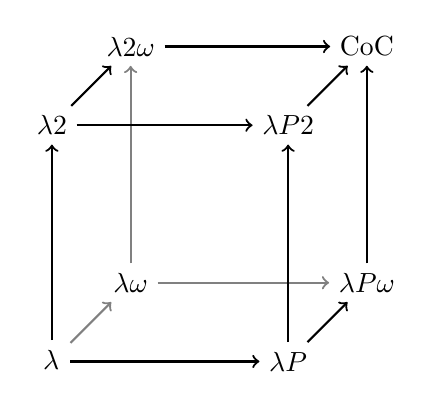
\begin{tikzpicture}
\node (A) at (0,0) {$\lambda_{\arrow}$};
\node (B) at (0,3) {$\lambda 2$};
\node (C) at (3,0) {$\lambda P$};
\node (D) at (1,1) {$\lambda\omega$};
\node (E) at (3,3) {$\lambda P2$};
\node (F) at (1,4) {$\lambda 2\omega$};
\node (G) at (4,1) {$\lambda P\omega$};
\node (H) at (4,4) {$\CC$};

\draw[->,thick,gray] (D) edge[<-] (A) edge (F) edge (G);
\draw[->,thick] (A) edge (B) edge (C)
                (B) edge (F) edge (E)
                (C) edge (G) edge (E)
                (F) edge (H)
                (E) edge (H)
                (G) edge (H);
\end{tikzpicture}
\end{center}

\newcommand{\SystemF}{\textsf{System F}}

The majority of this system has been studied (\todo{cite all papers paja}). 
The culmination of the \lambdaCube{}
is the Calculus of Construction (\CC{}) created by Coquand and Huet \cite{coqhuand:CoCIntro}. Here we have 
all abstractions: terms abstracted over types, types abstracted over types, and types abstracted over terms.

All the systems in \lambdaCube{} are known to have the strongly normalizable property and the are all
related to some logic: $\lambda 2$, also known as \SystemF{} introduced independently at 
\cite{girard:Paradox,Reynolds:systemFIntro}, is equivalent to second order logic, for example.

\subsection{Calculus of Constructions}
In \CC{}, the propositions (types) that can be stated are much more fine grained compared to the simply 
typed lambda calculus. This is due to the combination of dependent types, type constructor and type quantification,
which gives a very expressive framework to develop mathematics, via the Curry-Howard correspondence,
whose proof of propositions can be verified by a type system. Furthermore, because lambda 
calculus can also model programming languages, this gives a framework for establishing propositions over 
programs in the same language. 

\section{Calculus of Inductive Constructions}
\label{sec:CIC}
In this section we present the calculus of inductive constructions (\CIC{})
\cite{werner1994:IntroCIC,coqRef} in detail,
and how it can be used to develop mathematics from another perspective. The presentation we
give is by step, starting from a calculus without inductives but equal in every other aspect. Such calculus
is the predicative calculus of constructions (\CCw{}) which is an extension of \CC{} with a predicative 
sort \footnote{This will be defined in a moment}, much like
Luo's Extended Calculus of Construction \cite{Luo1994:ECC}
without $\Sigma$-types. 
% This calculus does not have an impredicative sort, so we include it. 
% This presentation is extracted from \cite{coqRef}.

\subsection{Terms} \todo{Quizas hablar sobre el ambiente global}
Terms represent the valid syntactical expressions of the calculus. \CIC{} was designed to not make a 
syntactic distinction between types and terms in the sense of simply typed lambda calculus. This decision
produce a problem though. Every term must have a type (a posteriori), but types do not type to anything yet.
It is naturally then to define the \emph{sorts}

\begin{Definition}[Sort] Sorts are the types of types.\end{Definition}
\noindent Because sorts can be seen as types, they also are a valid syntactic expression. More formally,
sorts are defined in \CCw{} as:
\begin{center}
    $\Sort{} = \{\Prop\} \cup \{\Type{}\ |\ i\in\Nat\} $
\end{center}
Here \Prop{}, readed as prop, represent the type of propositions and \Type{}, readed as universe,
represents the type of types. Note that types are accompanied by \emph{universe levels}, 
represented by $i$ in \Type{}. In \sectRef{CCw-TypeSystem} will be explained why is needed this structure. 
From now on, for every expression $\ctyping{A}{s}$ we assume that $s\in\Sort$.

As usual, we need to keep track of variables when typing abstractions. However, this approach does not allow
to view the type theory as a system. Instead of using the context only to type abstractions, we also add
the valid definitions. Also, we support the addition of assumptions. Definitions are represented by 
$(c:=M:T)$ and assumptions by $(c:T)$.
Although the contexts 
are not a syntactic construction, they are a sort of a meta-term used to type check. 

Recall in the untyped lambda calculus, we had defined the substitution by $\untypedSubst{t}{u}{x}$ in 
\defRef{def:untypedSubst}. Now we are 
going to redefine it with a different syntax, to make it more explicit, but keeping the same behavior, \ie{}, 
substitute only the free variables. The definition of free and bound variables are derived from 
\defRef{def:boundFreeVar}.
\begin{Definition}[Substitution: Redefinition]
Given terms $M$ and $N$, then $\subst{M}{x}{N}$ represents the term $M$ where all free occurrence of the 
variable $x$ are replaced by the term $N$.
\end{Definition}

To summarize, the valid syntactical expressions are: variables, lambda abstractions, applications, dependent
products and sort. In \figRef{fig:CCwExpression} is the syntax definition.

\begin{figure}
    \centering
    $A,B,C,D,I,N,M,R,S\ \termDef\ \Type\ |\ \Prop\ |\ x\ |\ \app{M}{N}\ |\ \abs{x}{A}{M}\ |\ \vardepArrow{A}{B}$\\
    \rule{0.75\textwidth}{0.4pt}\vspace{4pt}\\
    $\Context,\varContext\ \termDef\ \EContext\ |\ \Context,\typing{x}{A}\ |\ 
                                      \Context,\definitionWtype{x}{M}{A}$ %\vspace{4pt}\\
    %$\GContext \termDef \EContext\ |\ \GContext,\typing{x}{A}\ |\ \GContext,\typing{x\termDef M}{A}$
    \caption{Valid syntactic expression of \CCw{} + \Prop{}}
    \label{fig:CCwExpression}
\end{figure}

\subsection{Type system}
\label{CCw-TypeSystem}

We now have the valid syntactic expression that correspond to the calculus. We proceed to define
a type discipline over these expressions. This is done by defining simultaneously two judgments. 
The first one is \ctyping{M}{A} which establish that the term $M$ as type $A$ in the context \Context{} 
and the \wfContext{\Context} which establish that the context is valid.

We introduce the rules and give a brief explanation:
\newcommand{\CicWfEmpty}{\textsc{WF-Empty}}
\begin{mathpar}
\inferrule*[lab=\CicWfEmpty]{ }{\wfContext{[]}}
\end{mathpar}
This establish that an empty context is valid.

\newcommand{\CicWfHyp}{\textsc{WF-Hyp}}
\newcommand{\CicWfConst}{\textsc{WF-Const}}
\begin{mathpar}
\inferrule*[lab=\CicWfHyp]{\ctyping{A}{s} \and x\notin\Context}{\wfContext{\Context,\typing{x}{A}}}
\and 
\inferrule*[lab=\CicWfConst]{\ctyping{M}{A} \and x\notin\Context}{\wfContext{\Context,\definitionWtype{x}{M}{A}}}
\end{mathpar}
In the first case, we are adding an assumption to the context and in the second case a definition.

\newcommand{\CicType}{\textsc{Type}}
\newcommand{\CicProp}{\textsc{Prop}}
\begin{mathpar}
\inferrule*[lab=\CicType]{\wfContext{\Context}}{\ctyping{\Type[i]}{\Type[i+1]}}
\and 
\inferrule*[lab=\CicProp]{\wfContext{\Context}}{\ctyping{\Prop}{\Type[1]}}
\end{mathpar}
% The first rule define the cumulative structure of universes. Cumulative means that if the universe is smaller 
% (expressed by the rule $i<j$), then is contained in the bigger universe. 
The \CicType{} has this form to avoid the Girard's 
Paradox \cite{girard:Paradox}, which arises if we allowed $\typing{\Type[]}{\Type[]}$ (without universes).
Note that \Prop{} is contained in a universe and not in itself.

\newcommand{\CicVar}{\textsc{Var}}
\begin{mathpar}
\inferrule*[lab=\CicVar]{
    \wfContext{\Context} \and 
    (\typing{x}{A})\in\Context\text{ or }(\definitionWtype{x}{M}{A})\in\Context\text{ for some }M}{
    \ctyping{x}{T}}
\end{mathpar}
This rule establishes that assumptions or definitions in context can be derived.

\newcommand{\CicProdImpr}{\textsc{Prod-Impr}}
\newcommand{\CicProdForm}{\textsc{Prod-Form}}
\begin{mathpar}
    \inferrule*[lab=\CicProdImpr]{\ctyping{A}{s} \and \ctyping[\typing{x}{A}]{B}{\Prop}}{
               \ctyping{\depArrow{x}{A}{B}}{a}}
    \and
    \inferrule*[lab=\CicProdForm]{\ctyping{A}{\Type} \and \ctyping[\typing{x}{A}]{B}{\Type}}{
               \ctyping{\depArrow{x}{A}{B}}{\Type}}
    % \and
    % \inferrule*[lab=Prod-Type]{\ctyping{A}{\Type[j]} \and \ctyping[\typing{x}{A}]{B}{\Type[i]}}{
    %           \ctyping{\depArrow{x}{A}{B}}{\Type[max(i,j)]}}
\end{mathpar}
Here are the type judgments of the dependent product. Note the impredicativity of \CicProdImpr{}, \ie{},
the sort of the argument is not relevant.

\NewDocumentCommand{\convTyping}{O{\Context}m}{\ensuremath{#1\vdash#2}}
\renewcommand{\convertible}[3][\Context]{\ensuremath{\convTyping[#1]{#2\equiv#3}}}
\newcommand{\CicConv}{\textsc{Conv}}
\begin{mathpar}
    \inferrule*[lab=\CicConv]{\ctyping{M}{B} \and \ctyping{A}{s} \and \convertible{A}{B}}{
               \ctyping{M}{A}}
\end{mathpar}
This rule is the conversion rule. Intuitively, it allows to change the type of a term to another \emph{equal} type.
The notion of convertibility would be defined in \sectRef{section:CCwConversion}.

\newcommand{\CicLam}{\textsc{Lam}}
\newcommand{\CicApp}{\textsc{App}}
\begin{mathpar}
    \inferrule*[lab=\CicLam]{\ctyping[\typing{x}{A}]{M}{B} \and \ctyping{\depArrow{x}{A}{B}}{s}}{
               \ctyping{(\abs{x}{A}{M})}{\depArrow{x}{A}{B}}}
    \and
    \inferrule*[lab=\CicApp]{\ctyping{M}{\depArrow{x}{A}{B}} \and \ctyping{N}{A}}{
               \ctyping{(\app{M}{N})}{\subst{B}{x}{N}}}
\end{mathpar}

These judgments establish the type system over terms. We now proceed to explain what are conversion rules 
used to type check the \textsc{Conv} judgment.

\subsection{Conversion rules}
\label{section:CCwConversion}

Because types can depend on terms, it is necessary to allow \emph{computations} at the type level. For example, the 
following types are essentially the same, but differ in a syntactical manner:
\begin{center}
    $\app{(\abs{A}{\Type[i+1]}{A})}{\Type[i]}$ \hspace{2em} $\Type[i]$
\end{center}

We say that these types are intentionally equal, or convertible. The rules that establish that the previous 
types are convertible are the conversion rules and below we define all of them:

\begin{adjustwidth}{2em}{0cm}
\textDef{\betaRed{}} This rule was explained in the simple type lambda setting. Here, the properties of strong
normalization and confluence are inherited, being \CCw{} an extension of \CC{}.
\begin{center}
    $\convTyping{\reductionBeta{\app{(\abs{x}{A}{M})}{N}}{\subst{M}{x}{N}}}$
\end{center}

\textDef{\iotaRed{}} This rule of conversion is related to inductive types. It will be defined in 
\sectRef{subSect:InductiveTypes}.

\textDef{\deltaRed{}} Given a context under which variables may exists. This rules allows the identification
between the variable and its body, \ie{}, unfold the definition.
\begin{mathpar}
    \inferrule{\wfContext{\Context} \and (\typing{c\termDef M}{A})\in\Context}{
               \convTyping{\reductionDelta{x}{M}}}
\end{mathpar}

\textDef{\etaExp{}} This rule allows the identification of function terms with its expansion.
\begin{mathpar}
    \inferrule{\wfContext{\Context} \and (\typing{c\termDef M}{(\depArrow{y}{A}{B})})\in\Context}{
               \convTyping{\expansionEta{M}{\abs{x}{A}{(\app{M}{x}})}}}
\end{mathpar}
\end{adjustwidth}

\subsubsection{Convertibility}
We define \convTyping{\reductionStrat{M}{N}} as the compatible closure of \reduction{\beta\iota\delta}.
We say that two terms $M_1, M_2$ are $\beta\iota\delta\eta$-convertibles (\convertible{M_1}{M_2})
iff there exists some terms $N_1,N_2$ such that \convTyping{\reductionStrat{\reductionStrat{M_1}{\dots}}{N_1}}
and \convTyping{\reductionStrat{\reductionStrat{M_2}{\dots}}{N_2}} and either $N_1$ and $N_2$ are identical, or
they are convertible up to \etaExp{}

\subsection{Subtyping relation}
Up to now, we have not look at the cumulative property of \CIC{}, \ie{}, the property that a term that belongs
to a universe $i$ also belongs to the universe $j$ if $i<j$. This property extends the equivalance relation of 
convertibility to a subtyping relation. This relation is inductively defined by:
\newcommand{\subConvertible}[3][\Context]{\ensuremath{#1\vdash#2\leq#3}}
\begin{itemize}
\item If \convertible{A}{B}, then \subConvertible{A}{B}
\item If $i\leq j$, then \subConvertible{\Type}{\Type[j]}
\item For any $i$, then \subConvertible{\Prop}{\Type}
\item If \convertible{A}{B} and \subConvertible[\Context,\typing{x}{A}]{A'}{B'}, then
      \subConvertible{\depArrow{x}{A}{A'}}{\depArrow{x}{B}{B'}}
\end{itemize}
With this relation, the \CicConv{} rule is redifined as
\begin{mathpar}
\inferrule*[lab=\CicConv]{\ctyping{M}{B} \and \ctyping{A}{s} \and \subConvertible{A}{B}}{
               \ctyping{M}{A}}
\end{mathpar}

\subsection{Inductive types}
\label{subSect:InductiveTypes}
Until now, we have defined the valid expression and the type system of \CCw{}. \CIC{} is an extension of \CCw{},
where inductive types can be added to the language. However, the ability to add inductives to the language
does not give any extra power to the calculus at all, because inductives can be defined by their Church encoding
\todo{donde esta esto}. Nevertheless, in the latter approach is impossible to define the induction principle for 
inductives \cite{geuvers:IndNotDerivable2001}, while in \CIC{} is generated with a computational content. This
gives more power to \CIC{} in contrast to \CCw{}.

\subsubsection{Inductive introduction}
\newcommand{\CicIndWf}{\textsc{Ind-WF}}
\newcommand{\CicIndType}{\textsc{Ind-Type}}
\newcommand{\CicIndConstr}{\textsc{Ind-Constr}}
% IP = Inductive Parameters
% II = Inductive Indices
% IN = Inductive Name
% IT = Inductive Type
% IPN = Inductive Parameters Name
% IIN = Inductive Indices Name
% CT = Constructor Type
% CN = Constructor Name
\newcommand{\IP}{\ensuremath{P}}
\newcommand{\II}{\ensuremath{U}}
\newcommand{\IN}{\ensuremath{I}}
\newcommand{\IT}{\ensuremath{D}}
\newcommand{\IPN}{\ensuremath{p}}
\newcommand{\IIN}{\ensuremath{u}}
\newcommand{\CT}{\ensuremath{C}}
\newcommand{\CN}{\ensuremath{c}}

We proceed to define the syntax for declaring inductives and the type checking constraints that must satisfy 
so that they can be added to the context. Note that in \CIC{} is possible to define mutual inductive types.
\def\IndContextT{\ensuremath{\varContext_{I}}}
\def\IndContextC{\ensuremath{\varContext_{C}}}
\newcommand{\Constr}[2]{\ensuremath{\textsf{Constr}(#1,#2)}}

\begin{Definition}[Inductive Block]
\label{def:InductiveIntro}
Inductive definitions are introduced by inductive blocks. Inductive blocks
are of the form \IndIntro[n][\IndContextT][\IndContextC]{} where n represents the number of 
parameters of the types, 
\IndContextT{} the names of the inductives associated with their types and \IndContextC{} the constructors
of the inductives under definition associated with their types.
\end{Definition}
\noindent Note that \IndContextT{} and \IndContextC{} are contexts. In addition, \IN{} is used to identify an
inductive type and $c$ represents constructors.

In \figRef{fig:InductivesExample} we see examples of (mutual) inductive definitions represented as inductive 
blocks. Is important to note that this examples only represent syntax and additional checks are required 
for it to be valid.

\begin{figure}
    \begin{CoqDef}
    \\\IndIntro[0][
          \typing{\IndbadOne}{\Type[0]}][
          \typing{\text{bad1}}{\arrow{\IndbadOne}{(\arrow{(\arrow{\Indunit}{\IndbadOne})}{\Indunit})}{\IndbadOne}}]{}
    
    \IndIntro[1][
          \typing{\IndbadTwo}{\arrow{\Type}{\Type}}][
          \typing{\text{bad2}}{\app{\IndbadTwo}}{\Indunit}]{}
          
    \IndIntro[0][
          \typing{\IndbadThree}{\Type[0]}][
          \typing{\text{bad3}}{\IndbadOne}]{}
    
    \IndIntro[0][
              \typing{\Indnat}{\Type[0]}][
              \typing{\ConsO}{\Indnat},\typing{\ConsS}{\arrow{\Indnat}{\Indnat}}]
              
    \IndIntro[1][
              \typing{\Indvec}{\depArrow{A}{\Type}{\arrow{\Indnat}{\Type}}}][\\\hspace*{2em}
              \typing{\Consvnil}{\depArrow{A}{\Type}{\app{\Indvec}{A}{\ConsO}}},
              \typing{\Consvcons}{
                      \depArrow{A}{\Type}{n}{\Indnat}{\arrow{A}{
                                \app{\Indvec}{A}{n}}{\app{\Indvec}{A}{(\app{\ConsS}{n})}}}}]{}
    \IndIntro[0][
           \typing{\Indeven}{\arrow{\text{nat}}{\Type[0]}}, \typing{\Indodd}{\arrow{\text{nat}}{\Type[0]}}][
           \\\hspace*{2em}
           \typing{\text{even0}}{\app{\Indeven}{0}},
           \typing{\text{evenS}}{
                  \depArrow{n}{\text{nat}}{
                            \arrow{\app{\Indodd}{n}}{
                                   \app{\Indeven}{(\app{\text{S}}{n})}}}},\\\hspace*{2em}
            \typing{\text{oddS}}{
                    \depArrow{n}{\Indnat}{
                              \arrow{\app{\Indeven}{n}}{
                              \app{\Indodd}{(\app{\ConsS}{n})}}}}]
    \end{CoqDef}
    \caption{Examples of inductive definitions}
    \label{fig:InductivesExample}
\end{figure}

In order to maintain the logic consistency of the calculus, a restriction must be made over the structure of 
the inductives block. Thus, every time we declare an inductive block, we run a type check over the block
before adding the inductive types and their constructors to the context. Before giving the 
typing rules for inductives, is necessary the following definition.

\begin{Definition}[Arity of $s$] 
A type $A$ is said to be an arity of $s$, with $s\in\Sort$, if either $A$ is convertible to s or to a product
$\depArrow{x}{B}{A'}$ with $A'$ an arity of s.
\end{Definition}

\noindent From the previous definition, we say that a type $A$ is an arity if there exists some $s$ 
such as $A$ is an arity of $s$.

\begin{Definition}[Type constructor] 
We say that \CT{} is a type constructor of \IN{} if:
\begin{itemize}
\item \CT{} is ($\app{I}{R_1}{\dots}{R_n}$).
\item \CT{} is ($\depArrow{x}{A}{C'}$) where $C'$ is a type constructor of \IN{}.
\end{itemize}
\end{Definition}

\noindent From this we derive the concept of a constructor for a type \IN{}; 
if $(\typing{\CN}{\CT})\in\IndContextC$, then we say that \CN{} is a constructor of \IN{} iff \CT{} is a
type constructor of \IN{}. We see in \figRef{fig:InductivesExample}
that \CoqDefinition{even0} and \CoqDefinition{evenS} are constructors 
of \Indeven{}, and \CoqDefinition{oddS} is a constructor of \Indodd{}. In the \Indnat{} case,
both \ConsO{} and \ConsS{} are constructors of \Indnat{}.

The type checks are declared in \figRef{fig:CIC-Ind-rules} and are added to the \CCw{} ones
(extracted from \cite{timanySozeau:Consistency-pCuIC}). 

Note that in \CicIndWf{} rule we have a set $\Constr{\IndContextC}{\IN}$ which represent the constructors
of \IN{} in \IndContextC{}, and a new predicate 
\IndCheck{} that verify the following conditions:
\begin{itemize}
\item All variables in \IndContextT{} and \IndContextC{} are distinct

\item The first n arguments of all inductives and constructors of the block are the parameters. This means that 
there exists a sequence $\vv{\IP}$ such that $\textsf{len}(\vv{\IP})=n$ and for every
\mbox{$(\typing{x}{A})\in\IndContextT,\IndContextC$} we have that 
$\convertible{A}{\vvDepArrow{\IPN}{\IP}{B}}$ for some $B$. The notation $\typing{\vv{x}}{\vv{Y}}$ represents
$\typing{x_1}{Y_1},\dots,\typing{x_k}{Y_k}$ form some $k$.

\item For every $\IN\in\domContext{\IndContextT}$,
$(\typing{\CN}{\CT})\in\IndContextC$ and $\CN\in\Constr{\IndContextC}{\IN}$ we have that 
$\convertible{\CT}{\vvDepArrow{\IPN}{\IP}{\vvDepArrow{x}{A}{\app{\IN}{\vv{\IPN}}{\vv{v}}}}}$. Namely,
the parameters of the constructor must be passed to the inductive type definition. It is said that parameters are 
parametric. Note that the rest of the arguments passed to the inductive ($\vv{v}$) are not necessarily the same 
that the constructor receives ($\vv{x}$).

\item For every $(\typing{\IN}{\IT})\in\IndContextT$ we have that:
\begin{center}
$\convertible{\IT}{\vvDepArrow{\IPN}{\IP}{\vvDepArrow{\IIN}{\II}{s_{\IN}}}}$
\hspace{1em}
$\typing{\vvDepArrow{\IPN}{\IP}{\vvDepArrow{\IIN}{\II}{s_{\IN}}}}{s'_{\IN}}$
\end{center}
Here $\vv{\II}$ es the arity (or indices) of the inductive and $s_{\IN}$ its sort.

\item For every $\CN\in\domContext{\IndContextC}$, exists $\IN\in\domContext{\IndContextT}$ such that 
$\CN\in\Constr{\IndContextT}{\IN}$.

\item All inductive types in the block appear strictly positively in the constructor: \todo{define strictly
positive} see \cite{timanySozeau:Consistency-pCuIC} is different from \cite{coqRef} 
chapter \emph{Calculus of Inductive Constructions.Inductive Definitions}.
\end{itemize}

\begin{figure}
    \centering
    \begin{mathpar}
    \inferrule*[lab=\CicIndWf]{
        \IndCheck{} 
        \and 
        \ctyping{D}{s'_I}\text{ for all }(\typing{I}{D})\in\IndContextT
        \\\\
        \ctyping[\IndContextT]{C}{s_I}
            \text{ for all }(\typing{c}{C})\in\IndContextC\text{ if }c\in\Constr{\IndContextC}{I}
    }{
        \wfContext{\Context,\IndIntro[n][\IndContextT{}][\IndContextC{}]{}}
    }
    \and
    \inferrule*[lab=\CicIndType]{
        \wfContext{\Context} 
        \and 
        \IndIntro[n][\IndContextT][\IndContextC]\in\Context
        \and
        (\typing{I}{D})\in\IndContextT
    }{
        \ctyping{I}{D}
    }
    \and
    \inferrule*[lab=\CicIndConstr]{
        \wfContext{\Context} 
        \and 
        \IndIntro[n][\IndContextT][\IndContextC]\in\Context
        \and
        (\typing{c}{C})\in\IndContextT
    }{
        \ctyping{c}{C}
    }
    \end{mathpar}
    \caption{Type judgments for inductive blocks}
    \label{fig:CIC-Ind-rules}
\end{figure}


Coming back to \figRef{fig:InductivesExample}, we see that \IndbadOne{}, \IndbadTwo{}, \IndbadThree{}
are not valid definition blocks. The first one because it does not satisfy the positivity condition,
the second one because the constructor does not receive the parameters of the type and the third because
\CoqDefinition{bad3} is not a constructor for \IndbadThree{}.


\subsubsection{Inductive elimination}
% Predicate Name
\newcommand{\PredN}{\ensuremath{Q}} 
\newcommand{\CicIndElim}{\textsc{Ind-Elim}}

Until now, we have established how to introduce new inductive types, which also gives a form to construct them 
(by applying the constructors). However, is not possible to use (eliminate) them yet: check if a list is empty for 
example. We proceed to explain a way of doing this by adding a new syntactic term and new type judgments.

The main idea to eliminate a term whose type is an inductive one is to specify how it should behave for every 
constructor of the type, generating branches.
\begin{Definition}[Case block]
Inductive elimination is represented by \IndElim{\cdot}{\cdot}{\cdot|\dots |\cdot} where
the first argument is the inductive term, the second one a predicate over the term, and the third one represent
the branches for each constructor.
\end{Definition}

The predicate is a lambda whose arguments are the indices arguments of the inductive type plus the term of
the case. The type of the block case is the predicate applied the indices of the inductive and the term
itself.
Namely, given an inductive $\typing{\IN}{(\vvDepArrow{\IPN}{\IP}{\vvDepArrow{\IIN}{\II}{s_\IN}})}$, parameters
$\typing{\vv{a}}{\vv{\IP}}$, indices $\typing{\vv{i}}{\vv{\II}}$ and a term $M$ such as
$\ctyping{M}{\app{\IN}{\vv{a}}{\vv{i}}}$, then
the type of the predicate \PredN{} is 
$\enDepArrow{\vv{x}}{\subst{\vv{\II}}{\vv{\IPN}}{\vv{a}}}{\depArrow{x}{\app{\IN}{\vv{a}}{\vv{x}}}{R}}$
and the type of the block is $\app{Q}{\vv{i}}{\vv{M}}$

\todo{maybe speak about singleton elimination and allowed sort of elimination}

The branches of the block case represent what it should be done in case the term of the case was built by the 
specific constructor. This means that it must be one branch for every constructor. Specifically, the branches
are lambdas that take the non-parametric arguments of the respective constructor. 

In \figRef{fig:CaseTypeJudg} we can see the rule for typing a case block. This rule check that the 
predicate receives the indices of the inductive type along with a term that belongs to the inductive type itself.
Also check that each branch is well-typed respect to the predicate instantiated to the respective constructor 
and indices. Finally, the type of case block is the predicate applied to the indices of the term case 
and the term case itself.

Before showing some examples, is necessary to define \iotaRed{}. This reductions allows the identification
of a case block when applied on a specific constructor with its respective branch. Namely
\begin{center}
$\reductionIota{\IndElim{\app{\CN_i}{\vv{\IPN}}{\vv{\IIN}}}{\PredN}{f_1|\dots | f_l}}{\app{f_i}{\vv{\IIN}}}$
\end{center}

Now is possible to define terms wit the case block. For example, the following term 
verify if a list $\typing{l}{\app{\Indlist}{A}}$ is empty: 
\newcommand{\noBinder}{\rule{8pt}{1pt}}
\newcommand{\nonLambda}[1]{\ensuremath{\lambda\, \noBinder\,.\,#1}}
\begin{center}
    $\IndElim{l}{\nonLambda{\Indbool}}{\Construe\ |\ \Consfalse}$
\end{center}
Here the predicate is homogeneous across all branches, so it can be dummy over the arguments ($\nonLambda{M}$ 
stands the corresponding lambda, but their arguments are not binded, although in this case no binder is needed).
However, this is not always the case. For example, getting the head of a vector needs a smarter predicate. 
This function has the following signature:
\def\vecHead{\CoqDefinition{head}}
\begin{center}
$\typing{\vecHead}{\depArrow{n}{\Indnat}{A}{\Type}{v}{\app{\Indvec}{A}{(\app{\ConsS}{n})}}{A}}$    
\end{center}
Because there must be one branch per constructor, the naive definition of \vecHead{} is not enough:
\begin{center}
    $\IndElim{v}{\nonLambda{A}}{\Constt\ |\ \abs{n}{\Indnat}{a}{A}{v}{\app{\Indvec}{A}{n}}{a} }$
\end{center}
The previous case does not type check due to empty constructor of the vector, even though this case block 
is never applied to an empty vector. This is a sign that the predicate 
of the block needs to be refined: it depends on the indices of the inductive. Because the predicate can be
any term, it is possible to do a case analysis on the form of the indices of the type:
\begin{center}
    $\IndElim{v}{\depArrow{n}{\Indnat}{\noBinder}{\noBinder}{\IndElim{n}{\nonLambda{\Type}}{\Indunit|A}}}{
             \Constt\ |\ \abs{n}{\Indnat}{a}{A}{v}{\app{\Indvec}{A}{n}}{a}}$
\end{center}
We also know that the type of the case correspond to apply the predicate to the indices and the term:
\begin{center}
$\typing{\vecHead}{\depArrow{n}{\Indnat}{A}{\Type}{v}{\app{\Indvec}{A}{(\app{\ConsS}{n})}}{
        \app{(\abs{n}{\Indnat}{\noBinder}{\noBinder}{
                   \IndElim{n}{\lambda \_.\Type}{\Indunit|A}}}})}{(\app{\ConsS}{n})}{v}$
\end{center}
Doing some \betaRed{} we get:
\begin{center}
$\typing{\vecHead}{\depArrow{n}{\Indnat}{A}{\Type}{v}{\app{\Indvec}{A}{(\app{\ConsS}{n})}}{
                             \IndElim{(\app{\ConsS}{n})}{\lambda \_.\Type}{\Indunit|A}}}$
\end{center}
Applying \iotaRed{} gives the desired result 
\begin{center}
$\typing{\vecHead}{\depArrow{n}{\Indnat}{A}{\Type}{v}{\app{\Indvec}{A}{(\app{\ConsS}{n})}}{A}}$
\end{center}
By a similar process the branches of the outer case are well-typed.

\begin{figure}
\centering
\begin{mathpar}
\inferrule*[lab=\CicIndElim]{
    \wfContext{\Context}
    \and
    \IndIntro[n][\IndContextT][\IndContextC]\in\Context
    \and
    (\typing{\IN}{(\vvDepArrow{\IPN}{\IP}{\vvDepArrow{\IIN}{\II}{s_\IN}}}))\in\IndContextT
    \\\
    \{\CN_i\}_{i=1\dots l}\in\Constr{\IndContextC}{\IN}
    \and
    (\ctyping{\CN_i}{\vvDepArrow{\IPN}{\IP}{\vvDepArrow{x_i}{A_i}{\app{\IN}{\vv{a}}{\vv{v_i}}}}})_{i=1\dots l}
    \\\\
    \cvvtyping{a}{\IP}
    \and
    \ctyping{\vv{i}}{\subst{\vv{\II}}{\vv{\IPN}}{\vv{a}}}
    \and
    \ctyping{M}{\app{\IN}{\vv{a}}{\vv{i}}}
    \\\
    \ctyping{\PredN}{(\enDepArrow{\vv{y}}{\subst{\vv{\II}}{\vv{\IPN}}{\vv{a}}}{
                                  \depArrow{x}{\app{\IN}{\vv{a}}{\vv{y}}}{B}})}
    \and
    (\ctyping{f_i}{\enDepArrow{\vv{x_i}}{\subst{\vv{A_i}}{\vv{\IPN}}{\vv{a}}}{
                               \app{\PredN}{\vv{v_i}}{(\app{c_i}{\vv{p}}{\vv{x_i}})}}})_{i=1\dots l}
}{
\ctyping{\IndElim{M}{\PredN}{f_1|\dots|f_l}}{(\app{\PredN}{\vv{i}}{M})}
}
\end{mathpar}
\caption{Elimination of an inductive type}
\label{fig:CaseTypeJudg}
\end{figure}

\section{CIC Extensions}
Until now, we only stated that type sorts have a level: \Type[i]{} has level $i$, for example.
In practice, the calculus presented in \sectRef{sec:CIC} needs explicit levels at every type sort instantiation.
This explicit instantiation has some drawbacks: truly type polymorphic functions and cumulative inductives
are not supported. In the next sections we show extension to \CIC{} that solves the previous issues.

\subsection{Universe polymorphism}
As stated before, universe levels must be explicit. Given a fixed universe level $i$ such
that $0\leq i$, the following term is intended to represent an identity function for all types:
\begin{center}
\CoqDefinition{id} 
\termDef{} 
\typing{\abs{A}{\Type[i]}{a}{A}{a}}{(\typing{\depArrow{A}{\Type[i]}{\arrow{A}{A}})}{\Type[i+1]}}
\end{center}
With this definition, and because \typing{\Indnat}{\Type[0]}, the following is a valid application:
\begin{center}
\typing{(\app{\CoqDefinition{id}}{\Indnat})}{\arrow{\Indnat}{\Indnat}}
\end{center}
However, there is no level on which this definition is valid:
\begin{center}
\newcommand{\id}{\CoqDefinition{id}}
\app{\id}{(\depArrow{A}{\Type[i]}{\arrow{A}{A}})}{\id}
\end{center}
Because the calculus enforce $\Type[i+1]\leq\,\Type[i]$, which is not possible.
In \cite{UniversePoly}, they introduced universe polymorphism for a variant of \CIC{} where is possible 
to define terms that are truly type polymorphic, in the sense that types can be instantiated with
different levels at different times. This is accomplished by carrying a context of constraint for 
each definition, where the universe levels are declared with their constraints.
For example, the following term defines a truly polymorphic identity function:
\newcommand{\polyi}{\ensuremath{\underline{i}}}
\begin{center}
\CoqDefinition{pid} 
\termDef{} 
\typing{\abs{A}{\Type[\polyi]}{a}{A}{a}}{(\typing{\depArrow{A}{\Type[\polyi]}{\arrow{A}{A}})}{\Type[\polyi+1]}}
\end{center}
The context carried is simply the declaration of the polymorphic universe level \polyi{} with a constraint
$0\leq\polyi$.
This level can be instantiated at type application, so now is possible to self-apply, but it 
is necessary to explicit the level:
\begin{center}
\newcommand{\id}{\CoqDefinition{pid}}
\app{\id}{(\depArrow{A}{\Type[0]}{\arrow{A}{A}})}{\id} 
\\
\app{\id}{(\depArrow{A}{\Type[i]}{\arrow{A}{A}})}{\id}
\end{center}
Note that in both cases, the polymorphic level \polyi{} of the second \CoqDefinition{pid} is instantiated 
to 0 and $i$, respectively, which in turn instantiate the polymorphic level \polyi{} of the first one
to 1 and $i+1$.

\subsection{Cumulative inductives}
Another limitation that \CIC{} has, even when adding universe polymorphism, is that inductive type do not
form a cumulative relation. Note that talking about cumulativity only make sense in a polymorphic
context. The non-cumulativity of inductive types can be seen with the following example. 
Given two universe level $j$ and $k$ such that $j<k$, and a 
polymorphic inductive type 
\newcommand{\Indtest}{\CoqDefinition{test}}
\IndIntro[0][\typing{\Indtest}{\depArrow{A}{\Type[\polyi]}}{\Type[\polyi+1]}][
\typing{\CoqDefinition{ctest}}{\depArrow{A}{\Type[\polyi]}{\app{\Indtest}{A}}}]{},
then the following theorem is not provable:
\begin{center}
    $\depArrow{A}{\Type[j]}{H}{\app{\Indtest}{[j]}{A}}{\app{\Indtest}{[k]}{A}}$
\end{center}
where the brackets in the previous example corresponds to instantiation of universe level. Intuitively, 
this theorem should be provable because $\app{\Indtest}{[j]}{A} < \app{\Indtest}{[k]}{A}$ if 
$\Type[j]\leq\Type[k]$. This extension was developed by Timany and Sozeau 
\cite{timanySozeau:Consistency-pCuIC} where they demonstrated the consistency of this extensions.
Now we proceed to explain the typing extension in order to support this system.

\todo{Define the rules extension}

\newcommand{\pCuIC}{\text{pCuIC}}
From now on, every time we talk about \CIC{} we will be referring to the the predicative calculus 
of cumulative inductive constructions (\pCuIC{}) which correspond to \CIC{} plus the extension of 
universe polymorphism and cumulative inductives.

\subsection{Coq: The proof assistant}
\label{subsection:Coq}
\newcommand{\Coq}{\text{Coq}}
\Coq{} is a proof assistant that allows to the specification and the development of software in the same 
environment. \Coq{} implements \CIC{} which provides the tools for such an environment.
However, \Coq{} uses \CIC{} as the kernel for the its theory and provide higher abstraction layers on top of it
so it can be more user friendly. We proceed to explain how this two system relate.

First, it is necessary to define how are represented the terms of \CIC{} in \Coq{}. 
It is important to note that the terms of \Coq{} posses the same structure 
if the ones in \CIC{}. Instead of provide a the BNF syntax definition, it will be 
represented as representations. This can be seen in \figRef{fig:CoqCICRepr}.

{
\renewcommand{\arraystretch}{1.5}
\begin{figure}
    \centering
    \begin{tabular}{|c|c|}
    \hline
    \rowcolor[gray]{0.9}Term in \CIC{} & Term in \Coq{} \\
    \hline
    \Type & \VernacType[i] \\
    \hline
    \Prop & \VernacProp \\
    \hline
    \abs{x}{A}{M} & \lstCoqInline!fun (x: A) => M! \\
    \hline
    \arrow{A}{B} & \lstCoqInline!A -> B! \\ 
    \hline
    \multirow{2}{*}{\depArrow{x}{A}{B}} & \lstCoqInline!forall (x: A), B! \\
                                        & \lstCoqInline!$\forall$(x: A), B! \\
    \hline
    \end{tabular}    
    \caption{\Coq{} representations of \CIC{} terms without inductives}
    \label{fig:CoqCICRepr}
\end{figure}
}

\subsubsection{Typical ambiguity}
The type hierarchy requires explicit universe level. However, it is cumbersome to explicit each
level. This is the reason \Coq{} provides \emph{typical ambiguity} for every type use.
The concept typical ambiguity remount to Russel's type theory \cite{1908:Russel_TypeTheory} and 
here is used in a similar manner


\subsubsection{Commands}
\Coq{} allow the introduction of term and inductive definitions. The first one is done by 
\VernacDefinition{} and the second one by \VernacInductive{}. In 

\begin{figure}
    \centering
    \begin{minipage}{\textwidth*2/3}
    \begin{lstlisting}[language=Coq]
    Definition definition (A: Type) := A.
    Definition definition := fun (A: Type) => A.
    \end{lstlisting}
    \end{minipage}
    \caption{Example of \Coq{} definitions}
    \label{fig:CoqDefinitionExample}
\end{figure}




\todo{talk about typical ambiguity, how it tries to simulate universe polymorphism  and how the constructs of coq translate to CiC}

\section{Parametricity}
In this sections we are going to talk about parametricity. We present the introduction of the terminology,
how can be used to derive properties about the terms and how can be used in practice.

\subsection{The abstraction theorem}
\newcommand{\SetBool}{as}

In 1983, Reynolds \cite{Reynolds83:TypesAbstractionAndParametricPolymorphism} introduced \SystemF{} and
stated a property over the terms: expressions in related contexts will be related values. Reynolds called 
this property \emph{the abstraction theorem}. The interesting part of the theorem is that it allows 
to reason about polymorphic functions, \ie{}, terms of type $\forall X.T$. Note that in \SystemF{}, 
a function that is polymorphic must behave in the same way for all types instantiation. Nevertheless,
this theorem states that related terms will be related after the function application.

Reynolds formulated the abstraction theorem for a set theoretic construction

\subsection{Parametricity and free theorems}
The abstraction theorem was renamed to \emph{parametricity} by Wadler \cite{Wadler:1989:TheoremsForFree}.
Here Wadler derived theorems for polymorphic functions using only parametricity. As a consequence, 
these theorems holds for all types instantiation. For example

\subsection{Parametricity in dependent typed languages}

\section{Models and Syntactic Translation}
The lambda calculus is a good abstraction tool. However, it is .... A model for the lambda calculus 
provides \emph{meaning} to the well-typed terms of the calculus. There are plenty models for lambda 
calculus and their variants, including CIC \cite{timanySozeau:Consistency-pCuIC}. However, all this models
are in another theory outside if type theory. PIM \todo{fix} \cite{700syntactical}, proposed
to use as model \CIC{} itself. This gives a notation of compilation

\subsection{The exceptional translation}

\subsection{The parametric exception translation}
 

\chapter{New Parametric Exceptional Translation}
\label{ch:translation}

%\setcounter{page}{1}
%\setcounter{figure}{0}
%\setcounter{globDefs}{0}

\newcommand{\FreeVar}[1]{\mathtexttt{FreeVar}(#1)}

\newcommand{\ExceptionType}{\ensuremath{\mathbb{E}}}
\newcommand{\BExceptionType}{\text{\rmfamily \textbf{E}}}

\newcommand{\raiseFun}{\mathtexttt{raise}}
\newcommand{\unit}{\mathtexttt{unit}}
\newcommand{\ttUnit}{\mathtexttt{tt}}
\newcommand{\eqRefl}{\mathtexttt{refl}}


\renewcommand{\CicType}{\textsc{Type}}
\renewcommand{\CicProp}{\textsc{Prop}}
\newcommand{\CicWeak}{\textsc{Weakening}}
\newcommand{\CicTypeProd}{\textsc{Type-Prod}}
\newcommand{\CicPropProd}{\textsc{Prop-Prod}}
\newcommand{\CicImpred}{\textsc{Impred}}
\renewcommand{\CicConv}{\textsc{Conv}}
\newcommand{\CicAbs}{\textsc{Abs}}
\renewcommand{\CicApp}{\textsc{App}}
\newcommand{\CicIdem}{\textsc{Idem}}
\newcommand{\CicWfnil}{\textsc{Wf-Empty}}
\newcommand{\CicWfcons}{\textsc{Wf-Cons}}

In \todo{put ref} is presented a syntactic translation for \CIC{} that adds exception to the 
language. This translation breaks the logic consistency of the calculus. In \todo{put ref},
the logic consistency is recovered with parametricity techniques if the exceptions do not
flow at the top level.

The calculus used for the translation is not the same presented here but a variation. The 
variations only take part on the functional fragment of the calculus (calculus without the inductives).
We present it in \figRef{fig:CCw*}

\begin{figure}
    \begin{mathpar}
    A,B,N,M,R,S\ \termDef\ \Type\ |\ \Prop\ |\ x\ |\ \app{M}{N}\ |\ \abs{x}{A}{M}\ |\ \vardepArrow{A}{B} \\
    \Context,\varContext\ \termDef\ \EContext\ |\ \Context,\typing{x}{A} \\
    
    \inferrule*[lab=\CicType]{\wfContext{\Context} \and i<j}{\ctyping{\Type}{\Type[j]}}
    \and
    \inferrule*[lab=\CicProp]{\wfContext{\Context}}{\ctyping{\Prop}{\Type}}
    \and  
    \inferrule*[lab=\CicWeak]{\ctyping{M}{B} \and \and \ctyping{A}{s}}{\ctyping[\typing{a}{A}]{M}{B}}
    
    \\ 
    
    \inferrule*[lab=\CicTypeProd]{\ctyping{A}{\Type} \and \ctyping[\typing{x}{A}]{B}{\Type[j]}}{%
               \ctyping{\vardepArrow{A}{B}}{\Type[\text{max(i,j)}]}}
    \and
    \inferrule*[lab=\CicPropProd]{\ctyping{A}{\Prop} \and \ctyping[\typing{x}{A}]{B}{\Type}}{%
               \ctyping{\vardepArrow{A}{B}}{\Type}}
    
    \\
    
    \inferrule*[lab=\CicImpred]{\ctyping{A}{s} \and \ctyping[\typing{x}{A}]{B}{\Prop}}{%
               \ctyping{\vardepArrow{A}{B}}{\Prop}}
               
    \inferrule*[lab=\CicConv]{\ctyping{M}{B} \and \ctyping{A}{s} \and \convertible{A}{B}}{\ctyping{M}{A}}
    
    \\
    
    \inferrule*[lab=\CicAbs]{\ctyping[\typing{x}{A}]{M}{B} \and \ctyping{\vardepArrow{A}{B}}{s}}{%
               \ctyping{\abs{x}{A}{M}}{\vardepArrow{A}{B}}}
    \and
    \inferrule*[lab=\CicApp]{\ctyping{M}{\vardepArrow{A}{B} \and \ctyping{N}{A}}}{\ctyping{\app{M}{N}}{\subst{B}{x}{N}}}
    
    \\
    
    \inferrule*[lab=\CicWfnil]{ }{\wfContext{\EContext}} 
    \and 
    \inferrule*[lab=\CicWfcons]{\ctyping{A}{s}}{\wfContext{\Context,\typing{x}{A}}}
    \and
    \inferrule*[lab=\CicIdem]{\ctyping{A}{s}}{\ctyping[\typing{x}{A}]{x}{A}}
    
    \\
    
    \inferrule{ }{\convertible{\app{(\abs{x}{A}{M})}{N}}{\subst{M}{x}{N}}}
    \and
    \inferrule{ }{\convertible{M}{\abs{x}{A}{(\app{M}{x})}}}
    \\
    \inferrule{\convertible{M_1}{M_2}}{\convertible{\app{M_1}{N}}{\app{M_2}{N}}}
    \and
    \inferrule{\convertible{N_1}{N_2}}{\convertible{\app{M}{N_1}}{\app{M}{N_2}}}
    
    \end{mathpar}
    \caption{\CCw + \Prop}
    \label{fig:CCw*}
\end{figure}

% The exceptional translation is a syntactical translation of \CIC{} that adds exceptions to the language. 
% The formalization is done in two stages. First, over a \CCw{}, which is similar to \CC{} with a cumulative 
% universe instead of the impredicative, and 
% then over the same language adding inductives. The underlying calculus \CCw{} is presented in \figRef{fig:CCw*}, 
% with the impredicative sort added. Here we have a set $\Sort\termEq \{\Prop\}\cup\{\Type{} |\ i\in\Nat\}$ and 
% $s\in\Sort$ for every $s$ in the definition.

From now on we define \Theory{} a theory that interprets \CIC{}, \ETheory{} the exceptional translation of 
\Theory{} and \PTheory{} the parametric exceptional translation of \Theory{}.

In \ETheory{} it is possible to define a new type \BExceptionType{} which exposes the underlying 
exceptional type \ExceptionType{} of the translation.
\begin{center} 
$\Trans{\BExceptionType}\termDef \app{\TypeVal}{\ExceptionType}{(\abs{e}{\ExceptionType}{e})}$ 
\end{center}
With this type, it is possible to define in \ETheory{} a function that inhabits any type providing a term
belonging to the 
exception $\typing{\raiseFun{}}{\depArrow{A}{\Type[]{}}{\arrow{\BExceptionType}{A}}}$ by:
\begin{center}
$\Trans{\raiseFun}\termDef \abs{A}{\TypeTrans{\Type[]{}}}{e}{\ExceptionType}{\app{\Err}{A}{e}}$ 
\end{center}
However, these previously defined terms do not belong to \PTheory, because both terms do not admit a 
parametric translation over \ParamTrans{\cdot}. Intuitively, \ParamTrans{\cdot} recursively verifies that 
a term is composed only by pure terms. Thus, it is not possible to establish parametric proofs that use 
impure programs, ie, these terms belong only to \ETheory{} but not to \PTheory. In the following 
example $\ExceptionType\termDef\unit$:
\begin{center}
$\exists (n:\mathtexttt{nat}),\ (\app{\raiseFun}{\ttUnit}) = n $
\end{center}
Given the definition of equality, existencial and natural in \figRef{fig:EqAndExDefs}, the proposition admits two
proofs in \ETheory{}:
\begin{center}
$(\app{\mathtexttt{intro}}{\mathtexttt{nat}}{(\abs{n}{\mathtexttt{nat}}{(\app{\raiseFun}{\ttUnit}) = n})}{
      (\app{\raiseFun}{\ttUnit})}{\eqRefl})$
\hspace{2em} 
$(\app{\raiseFun}{\ttUnit})$
\end{center}
It is desirable that the parametric translation allows the former, but prohibits the latter because 
the first establishes a property for the exceptional term while the second is an impure proof. Currently,
both terms are rejected because $(\app{\raiseFun}{\ttUnit})$ is used. 

\begin{figure}
\begin{CoqDef}%{\par\bfseries\ttfamily\noindent%
\IndIntro[2][\typing{\Indeq}{\depArrow{A}{\Type}{x}{A}{\arrow{A}{\Prop}}}][
             \typing{\Consrefl}{\depArrow{A}{\Type}{x}{A}{\app{\Indeq}{A}{x}{x}}}]

\noindent
\IndIntro[2][\typing{\Index}{\depArrow{A}{\Type}{P}{\arrow{A}{\Prop}}{\Prop}}][
             \typing{\Consintro}{\depArrow{A}{\Type}{P}{\arrow{A}{\Prop}}{
                                           \depArrow{x}{A}{p}{\app{P}{x}}{\app{\Index}{A}{P}}}}]
\end{CoqDef}%}%
    \caption{Inductive definitions}
    \label{fig:EqAndExDefs}
\end{figure}

Here we present a new syntactical 
translation over \CIC{} which is a variant of the exceptional one,
the \emph{weakly parametric exceptional translation} \WParamTrans{\cdot},
that relaxes the translation
over propositions and allows reasoning over impure programs, but prohibits impure proofs, \ie{}, 
accept the first proof and reject the second. 

\section{Translation for the Functional Fragment}

The exceptional translation transforms the sort hierarchy to a type hierarchy with a default exceptional
constructor:
\begin{itemize}
    \item $\Trans{\Type} \equiv \app{\TypeVal}{ \type}{\TypeErr} $
    \item $\Trans{\Prop} \equiv \app{\TypeVal}{ \prop}{\PropErr} $
\end{itemize}
\newcommand{\wSymbol}{\ensuremath{\omega}}
\NewDocumentCommand{\WTrans}{D<>{\Context}om}{%
    \ensuremath{[#3]^{#1\IfValueT{#2}{,#2}}_{\wSymbol}}%
}
\NewDocumentCommand{\WTypeTrans}{D<>{\Context}om}{%
    \ensuremath{[\![#3]\!]^{#1\IfValueT{#2}{,#2}}_{\wSymbol}}%
}
\NewDocumentCommand{\WTransErr}{D<>{\Context}om}{%
    \ensuremath{[#3]^{#1\IfValueT{#2}{,#2}}_{\wSymbol\,\phi}}%
}
\NewDocumentCommand{\WContextTrans}{m}{\WTypeTrans<>{#1}}
\renewcommand{\WTermTrans}[1]{\ensuremath{#1_{\wSymbol}}}

Both sorts can be inhabited by an exception in \ETheory{} providing an inhabitant
of \ExceptionType{}. We want to enforce the purity of the propositions, so the new translation
\WTrans{\cdot}
treats the propositional sort a little different 
\begin{center}
$\WTrans<>{\Prop} \equiv \app{\TypeVal}{\Prop}{(\varabs{_}{\ExceptionType}{\depArrow{A}{\Prop}{A}})} $
\end{center}
The default exceptional constructor for this case is chosen degenerated because in essence is never used in a 
meaningful way. Note that this new translation is not homogeneous, in the sense that 
the translation for the sorts differ in a fundamental way. As a consequence, it is necessary to tag
every term with the sort they belong to. This can be achieved by keeping an environment along the
translation. With this change, the new translation is defined in 
\figRef{fig:weaklyParExcTransDef}.

\begin{figure}
    \centering
    \begin{minipage}{\textwidth}
    \renewcommand{\arraystretch}{1.15}
    \begin{tabular}{l@{$\hspace{0.1em}\termDef$\ \ }l}
    \WTrans{\Type} & $\app{\TypeVal}{\type}{\TypeErr}$ \\
    \WTrans{\Prop} & $\app{\TypeVal}{
                           \Prop}{
                           (\abs{\noBinder}{\ExceptionType}{ (\depArrow{A}{\Prop}{A}) })}$ \\
    \WTrans{x} & $x$ \\
     
    \WTrans{\abs{x}{A}{M}} & $\abs{x}{\WTypeTrans{A}}{\WTrans[\typing{x}{A}]{M}}$ \\
    \WTrans{\app{\M{}}{\N{}}} & $\app{\WTrans{M}}{\WTrans{N}}$ \\
    \WTrans{\depArrow{x}{A}{B}} & $\! \! \left \{ \begin{matrix*}[l]
                                      \depArrow{x}{\WTypeTrans{A}}{\WTypeTrans[\typing{x}{A}]{B}}
                                       &
                                            \ctyping{\depArrow{x}{A}{B}}{\Prop} \\
                                      \app{\TypeVal}{
                                        (\depArrow{x}{\WTypeTrans{A}}{\WTypeTrans[\typing{x}{A}]{B}})
                                      }{
                                        (\abs{e}{\ExceptionType}{x}{\WTypeTrans{A}}{
                                              \app{\WTransErr[\typing{x}{A}]{B}}{e}})
                                      }
                                        & \otherwise
                                      \end{matrix*} \right.$ \\
    \WTransErr{A} & \app{\Err}{\WTrans{A}} \\
    \WTypeTrans{A} & $\! \! \left \{ \begin{matrix*}[l]
                                     \WTrans{A} & \ctyping{A}{\Prop} \\
                                      \app{\El}{\WTrans{A}} & \otherwise
                                      \end{matrix*} \right.$ \\
    \hline
    \rule{0pt}{15pt} \WContextTrans{\EContext} & \EContext \\
    \WContextTrans{\Context, \typing{x}{A}} &     
                $\WContextTrans{\Context},\typing{x}{\WTypeTrans<\Context>{A}}$
    \end{tabular}
    \end{minipage}
    \caption{Weakly Parametric Exceptional Translation}
    \label{fig:weaklyParExcTransDef}
\end{figure}

The translation is composed by four parts: \WTrans{\cdot} is used at the \emph{term} level, 
\WTypeTrans{\cdot} at the type level, \WContextTrans{\cdot} for contexts and \WTransErr{\cdot} for 
generating the exceptional default constructor. In figure \figRef{fig:translation_difference}
we can see the difference between both translations.
Note that reductions are applied in figure in order to be more concise.
Here we can see that if we restrict the calculus with only the \Type[]{} sort, then both translations
are equivalent. The translation remains almost unchanged with the new translation of \Prop{}. The interesting 
case is when the term being translated types to \Prop{}, which correspond to the last example in both examples.
The term and type translation are equal is this case (this are the branches in 
\figRef{fig:weaklyParExcTransDef}). Essentially, here is were the translation enforces the fact that 
propositions must remains pure in the exceptional layer. If a term types to \Prop{}, 
then in the translation 
it will also translate to \Prop{}, where no special machinery is defined to be able to raise an exception. 
Note that the \raiseFun{} term uses the second argument of \TypeVal{} to inhabit any type but for \Prop{}
such function does not exist.

\begin{figure}
\def\arraystretch{1.5}
\centering
\subfloat[][Translation for \Trans{\cdot}/\TypeTrans{\cdot}]{
\begin{tabular}{lll}
    \cline{2-3}
    & \Trans{\cdot} & \TypeTrans{\cdot} \\
    \hline
    % --------------------------
    \Type
    & 
    \app{\TypeVal}{\type}{\TypeErr}
    &
    \type \\
    % --------------------------
    \Prop
    & 
    \app{\TypeVal}{\prop}{\PropErr}
    &
    \prop \\
    % --------------------------
    \arrow{\Type}{\Type[j]}
    & 
    \app{\TypeVal}{
        (\arrow{\type}{\type[j]})}{
        (\abs{e}{\ExceptionType}{t}{\type}{\TypeErr})} 
    &
    \arrow{\type}{\type[j]} \\
    % --------------------------
    \arrow{\Type}{\Prop}
    & 
    \app{\TypeVal}{
        (\arrow{\type}{\prop})}{
        (\abs{e}{\ExceptionType}{t}{\type}{\PropErr})}
    &
    \arrow{\type}{\prop} \\
    % --------------------------
    \depArrow{A}{\Prop}{A}
    & 
    \app{\TypeVal}{
        (\depArrow{A}{\prop}{A})}{
        (\abs{e}{\ExceptionType}{A}{\prop}{\PropErr})} 
    &
    \depArrow{A}{\prop}{A} \\
    \hline
\end{tabular}
}

\subfloat[][Translation for \WTrans{\cdot}/\WTypeTrans{\cdot}]{
\begin{tabular}{lll}
    \cline{2-3}
    & \WTrans{\cdot} & \WTypeTrans{\cdot} \\
    \hline
    % --------------------------
    \Type
    & 
    \app{\TypeVal}{\type}{\TypeErr}
    &
    \type \\
    % --------------------------
    \Prop
    & 
    \app{\TypeVal}{\Prop}{(\depArrow{A}{\Prop}{A})}
    &
    \Prop \\
    % --------------------------
    \arrow{\Type}{\Type[j]}
    & 
    \app{\TypeVal}{
        (\arrow{\type}{\type[j]})}{
        (\abs{e}{\ExceptionType}{t}{\type}{\TypeErr})} 
    &
    \arrow{\type}{\type[j]} \\
    % --------------------------
    \arrow{\Type}{\Prop}
    &
    \app{\TypeVal}{
        (\arrow{\type}{\Prop})}{
        (\abs{e}{\ExceptionType}{t}{\type}{\depArrow{A}{\Prop}{A}})} 
    & 
    \arrow{\type}{\Prop} \\
    % --------------------------
    \depArrow{A}{\Prop}{A} 
    & 
    \depArrow{A}{\Prop}{A}
    &
    \depArrow{A}{\Prop}{A} \\
    \hline
\end{tabular}
}
    \caption{Difference between the translations}
    \label{fig:translation_difference}
\end{figure}

\begin{Lemma}
\label{lemma:wtrans_sort_involutive}
Given a context \Context{}, a term $M$ and a sort $s$ such that 
\ctyping[][\WContextTrans{\Context}]{\WTrans{M}}{\WTypeTrans{s}}, then 
\ctyping[][\WContextTrans{\Context}]{\WTypeTrans{M}}{s}.
\end{Lemma}

\begin{Proof}
By a case analysis over $s$.
\begin{ProofCase}{$s \termDef \Type$}
After reduction, we have to prove $\ctyping[][\WContextTrans{\Context}]{\app{\El}{\WTrans{M}}}{s}$
given $\ctyping[][\WContextTrans{\Context}]{\WTrans{M}}{\type}$. Because \El{} has type
$\arrow{\type}{\Type}$, the result is obtained by an application of the \CicApp{} rule.
\end{ProofCase}

\begin{ProofCase}{$s \termDef Prop$}
After reduction, we have to prove $\ctyping[][\WContextTrans{\Context}]{\WTrans{M}}{\Prop}$
given $\ctyping[][\WContextTrans{\Context}]{\WTrans{M}}{\Prop}$, which is trivial.
\end{ProofCase}
\end{Proof}

\begin{Lemma}[Substitution]
\label{lemma:wtrans_substitution}
Given a context \Context{} and terms $M$ and $N$, we have:
\begin{center}
    $\WTrans{\subst{M}{x}{N}} \equiv \subst{\WTrans{M}}{x}{\WTrans{N}}$
\end{center}
\end{Lemma}

\begin{Proof}
By induction on $M$ over a generalized context
\begin{ProofCase}{$M \termDef x, M \termDef y$}
These cases are trivial
\end{ProofCase}

\begin{ProofCase}{$M \termDef \Type, M \termDef \Prop$}
These cases are also trivial because $x$ is not involved in the translated term
\end{ProofCase}

\begin{ProofCase}{$M \termDef \app{M_1}{M_2}$}
We have $\WTrans{\subst{(\app{M_1}{M_2})}{x}{N}}$. We get by unfold the definition of substitution and 
the translation
\begin{center}
$\WTrans{\subst{(\app{M_1}{M_2})}{x}{N}}$ 
\\ $\equiv$ \\
$\WTrans{
    \app{(\subst{M_1}{x}{N})}{(\subst{M_2}{x}{N})}
}$
\\ $\equiv$ \\
$\app{
    \WTrans{\subst{M_1}{x}{N}}
}{
    \WTrans{\subst{M_2}{x}{N}}
}
$
\end{center}
It is possible to apply the induction hypothesis over $M_1$ and $M_2$
\begin{center}
$\app{
    (\subst{\WTrans{M_1}}{x}{\WTrans{N}})
}{
    (\subst{\WTrans{M_2}}{x}{\WTrans{N}})
}$
\end{center}
and by folding the definition of substitution and the translation
\begin{center}
$\app{
    (\subst{\WTrans{M_1}}{x}{\WTrans{N}})
}{
    (\subst{\WTrans{M_2}}{x}{\WTrans{N}})
}$
\\ $\equiv$ \\
$\subst{(\app{\WTrans{M_1}}{\WTrans{M_2}})}{x}{\WTrans{N}}$
\\ $\equiv$ \\
$\subst{\WTrans{\app{M_1}{M_2}}}{x}{\WTrans{N}}$
\end{center}
which is the required result.
\end{ProofCase}

\begin{ProofCase}{$M \termDef \abs{x}{A}{M_1}$}
Note that in this case the binder is the same being substituted. By unfolding the definition of
substitution and the translation, we get
\begin{center}
$\WTrans{
    \abs{x}{\subst{A}{x}{N}}{M_1}
}$
\\ $\equiv$ \\
$\abs{x}{\WTypeTrans{\subst{A}{x}{N}}}{\WTrans[\typing{x}{A}]{M_1}}$
\end{center}
It is necessary to do a case analysis over $\ctyping{\subst{A}{x}{N}}{s}$, with $s$ a sort,
to unfold $\WTypeTrans{\subst{A}{x}{N}}$ which could give either:
\begin{itemize}
\item \WTrans{\subst{A}{x}{N}}
\item \app{\El}{\WTrans{\subst{A}{x}{N}}}
\end{itemize}
In both cases, it follows directly that 
$\WTypeTrans{\subst{A}{x}{N}} \equiv \subst{\WTypeTrans{A}}{x}{\WTrans{N}}$
by using the induction hypothesis and unfolding/folding. Then, the conclusion can be established.
\end{ProofCase}

\begin{ProofCase}{$M \termDef \abs{y}{A}{M_1}$}
The binder in this case is distinct from the one being substituted. Nevertheless, it is possible 
to derive, unfolding the substitution just like in the previous case:
\begin{center}
\varabs{y}{\subst{\WTypeTrans{A}}{x}{\WTrans{N}}}{\WTrans[\typing{y}{A}]{\subst{M}{x}{N}}}
\end{center}
Here is possible to apply the induction hypothesis over \WTrans[\typing{y}{A}]{\subst{M}{x}{N}}, 
because the context can be instantiated arbitrarily,
\begin{center}
    \subst{\WTrans[\typing{y}{A}]{M}}{x}{\WTrans[\typing{y}{A}]{N}}
\end{center}
Additionally, we can assume that $y\notin\FreeVar{N}$ due to alpha rename which implies 
\begin{center}
$
\WTrans[\typing{y}{A}]{N}
\equiv
\WTrans{N}
$
\end{center}
because the context is used to type terms on two places and in those places is 
possible to do an inversion over the derivation and \Context{} can be used instead of 
\Context{},\typing{y}{A}. Then, by a folding of the translation we obtain
\begin{center}\subst{\WTrans{\abs{y}{A}{M}}}{x}{\WTrans{N}}\end{center}
\end{ProofCase}

\begin{ProofCase}{$M \termDef \depArrow{y}{A}{B}$}
It is necessary to do a case analysis over \ctyping{\subst{\depArrow{y}{A}{B}}{x}{N}}{s},
for $s$ a sort.
\begin{SubProofCase}{$s \termDef \Prop$}
We have in this case after reduction
\begin{center}
$\depArrow{y}{\WTypeTrans{\subst{A}{x}{N}}}{\WTypeTrans[\typing{y}{A}]{\subst{B}{x}{N}}}$
$\equiv$
$\depArrow{y}{\WTypeTrans{\subst{A}{x}{N}}}{\WTrans[\typing{y}{A}]{\subst{B}{x}{N}}}$
\end{center}
where the last equivalence holds because $\ctyping[\typing{x}{A}]{B}{\Prop}$. In this scenario,
the remaining of the subcase is equal to the lambda case.
\end{SubProofCase}

\begin{SubProofCase}{$s \termDef \Type$}
We have in this case after reduction
\begin{center}
$\app{\TypeVal}{M_1}{M_2}$
\end{center}
with
\begin{itemize}
\item $M_1 \termDef \depArrow{y}{\WTypeTrans{\subst{A}{x}{N}}}{
                            \WTypeTrans[\typing{y}{A}]{\subst{B}{x}{N}}}$
\item $M_2 \termDef \abs{e}{\ExceptionType}{y}{\WTypeTrans{\subst{A}{x}{N}}}{
                            \app{\WTransErr[\typing{y}{A}]{\subst{B}{x}{N}}}{e}}$
\end{itemize}
Both cases were solved previously by an unfolding, induction 
hypothesis application and folding again.
\end{SubProofCase}
Note that here no distinction were made between the binder being substituted and the one binding.
That is because the treatment is similar to what we did in the lambda case
\end{ProofCase}
\end{Proof}

\begin{Lemma}[Conversion]
\label{lemma:wtrans_conversion}
Given a context \Context{} and terms $M$ and $N$, if \convertible{M}{N} then 
\convertible{\WTrans{M}}{\WTrans{N}}
\end{Lemma}

\begin{Proof}
By induction over the conversion.
\begin{ProofCase}{\betaRed{}}
Here we have
\begin{itemize}
\item $M \termDef \app{(\abs{x}{A}{M_1})}{N_1}$
\item $N \termDef \subst{M_1}{x}{N_1}$
\end{itemize}
Unfolding the translation and applying \lemmaRef{lemma:wtrans_substitution}:
\begin{itemize}
\item $\app{(\abs{x}{\WTypeTrans{A}}{
                    \WTrans[\typing{x}{A}]{M_1}})}{\WTrans{N_1}}$
\item $\subst{\WTrans[\typing{x}{A}]{M_1}}{x}{\WTrans{N}}$
\end{itemize}
With these terms is possible to establish conversion between the two.
\end{ProofCase}

\begin{ProofCase}{\etaExp{}}
Here we have
\begin{itemize}
\item $M \termDef M_1$
\item $N \termDef \abs{x}{A}{(\app{M_1}{x})}$
\end{itemize}
Unfolding the translation:
\begin{itemize}
\item $\WTrans{M_1}$
\item $\abs{x}{\WTypeTrans{A}}{(\app{\WTrans{M_1}}{x})}$
\end{itemize}
Same as before, it is possible to establish the conversion between the two terms.
\end{ProofCase}

\begin{ProofCase}{App}
Without loss of generality, we can set that the conversion is established for 
left term of the application. The other case is similar. We have
\begin{itemize}
\item $M \termDef \app{M_1}{N'}$
\item $N \termDef \app{M_2}{N'}$
\end{itemize}
with \convertible{M_1}{M_2}. Unfolding the translation we get:
\begin{itemize}
\item $\app{\WTrans{M_1}}{\WTrans{N'}}$
\item $\app{\WTrans{M_2}}{\WTrans{N'}}$
\end{itemize}
Applying the induction hypothesis allows the conclusion.
\end{ProofCase}

\end{Proof}

The typing soundness theorem is, taking in consideration the previous discussion:
\begin{Theorem}
Given \Context, $M$, and $A$ with \wfContext{\Context} and \ctyping{M}{A}, then we have
\ctyping[][\WContextTrans{\Context}]{\WTrans{M}}{\WTypeTrans{A}}
\end{Theorem}

\begin{Proof}
By a mutual induction over the typing derivation.
\begin{ProofCase}{\CicType}
We need to prove 
$\ctyping[][\WContextTrans{\Context}]{
          \app{\TypeVal}{\type}{\TypeErr}}{
          \type[j]}$. 
We now that \TypeVal{} has type 
$\depArrow{A}{\type[i']}{\arrow{\arrow{\ExceptionType}{A}}{\type[i']}}$ and \type{} has type 
$\Type[j]$ with $i<j$. By a double \CicApp{}, we can conclude the result unifying $j$ with $i'$.
\end{ProofCase}

\begin{ProofCase}{\CicProp}
We need to prove 
$\ctyping[][\WContextTrans{\Context}]{
          \app{\TypeVal}{\Prop}{(\depArrow{A}{\Prop}{A})}}{
          \type}$. 
This is similar to the previous case.
\end{ProofCase}

\begin{ProofCase}{\CicWeak}
We need to prove 
$\ctyping[\typing{a}{\WTypeTrans{A}}][\WContextTrans{\Context}]{
          \WTrans{M}}{
          \WTypeTrans{B}}$. 
By the induction hypothesis we have $\ctyping[][\WContextTrans{\Context}]{
          \WTrans{M}}{
          \WTypeTrans{B}}$. It only remains to show
$\ctyping[][\WContextTrans{\Context}]{\WTypeTrans{A}}{s'}$ for some $s'$. We proceed by 
a case analysis over $s$
\begin{SubProofCase}{$s \equiv \Prop{}$}
We have $\ctyping[][\WContextTrans{\Context}]{\WTrans{A}}{\Prop}$ by the induction hypothesis
and also $\WTypeTrans{A}\equiv\WTrans{A}$. We get the result by applying \CicWeak{} with 
$s'\equiv\Prop$.
\end{SubProofCase}

\begin{SubProofCase}{$s \equiv \Type$}
We have $\ctyping[][\WContextTrans{\Context}]{\WTrans{A}}{\type[s']}$ by the induction hypothesis
and also $\WTypeTrans{A}\equiv\app{\El}{\WTrans{A}}$. In order to conclude, we need that 
$\ctyping[][\WContextTrans{\Context}]{\app{\El}{\WTrans{A}}}{s'}$. Recall that
\El{} has type \arrow{\type}{\Type}. By \CicApp{} on \app{\El}{\WTrans{A}}, we derive it 
types to \Type[s']. It is possible to conclude by \CicWeak{} on the previous results unifying
the universe levels.
\end{SubProofCase}
\end{ProofCase}

\begin{ProofCase}{\CicTypeProd}
We need to prove 
\begin{center}
$\ctyping[][\WContextTrans{\Context}]{
    \app{\TypeVal}{
        (\depArrow{x}{\WTypeTrans{A}}{\WTypeTrans[\typing{x}{A}]{B}}) 
        }{
        (\abs{e}{\ExceptionType}{x}{\WTypeTrans{A}}{\app{\WTransErr[\typing{x}{A}]{B}}{e}})
        }
    }{
    \type[max(i,j)]
    }$. 
\end{center}
If the first argument of \TypeVal{} types to $\type[max(i,j)]$ and the second to 
$(\depArrow{x}{\WTypeTrans{A}}{\WTypeTrans[\typing{x}{A}]{B}})$, we can conclude the proof
with a double application of \CicApp{} rule which gives the desired type. We proceed to 
check the first argument.

\noindent By the induction hypothesis we know that:
\begin{itemize}
\item $\ctyping[][\WContextTrans{\Context}]{\WTrans{A}}{\type}$
\item $\ctyping[\typing{x}{\WTypeTrans{A}}][\WContextTrans{\Context}]{
                \WTrans[\typing{x}{A}]{B}}{\type[j]}$
\end{itemize}
We can derive from these hypothesis the followings:
\begin{itemize}
\item $\ctyping[][\WContextTrans{\Context}]{\WTypeTrans{A}}{\Type}$
\item $\ctyping[\typing{x}{\WTypeTrans{A}}][\WContextTrans{\Context}]{
                \WTypeTrans[\typing{x}{A}]{B}}{\Type[j]}$
\end{itemize}
by expanding the definition of \WTypeTrans{\cdot} and applying \CicApp{} rule
over \El{} and \WTrans{\cdot} in both cases. By \CicTypeProd{} rule we get
\begin{center}
$\ctyping[][\WContextTrans{\Context}]{
    \depArrow{x}{\WTypeTrans{A}}{\WTypeTrans[\typing{x}{A}]{B}}}{
    \Type[max(i,j)]}$
\end{center}
It remains to show that 
\begin{center}
$\ctyping[][\WContextTrans{\Context}]{
    (\abs{e}{\ExceptionType}{x}{\WTypeTrans{A}}{\app{\WTransErr[\typing{x}{A}]{B}}{e}})
    }{
    (\arrow{\ExceptionType}{\depArrow{x}{\WTypeTrans{A}}{\WTypeTrans[\typing{x}{A}]{B}}})
}$
\end{center}
which can be reduced to prove the body of the lambda
\begin{center}
$\ctyping[\typing{e}{\ExceptionType},\typing{x}{\WTypeTrans{A}}][\WContextTrans{\Context}]{
    (\app{\WTransErr[\typing{x}{A}]{B}}{e})
    }{
    \WTypeTrans[\typing{x}{A}]{B}
}$
\end{center}
We have $\app{\WTransErr[\typing{x}{A}]{B}}{e} \equiv \app{\Err}{\WTrans[\typing{x}{A}]{B}}{e}$ 
by definition, and $\typing{\Err}{\depArrow{A}{\type}{\arrow{\ExceptionType}{\app{\El}{A}}}}$.
Applying \CicApp{} two times we get 
\begin{center}
$\ctyping[\typing{e}{\ExceptionType},\typing{x}{\WTypeTrans{A}}][\WContextTrans{\Context}]{
    (\app{\Err}{\WTrans[\typing{x}{A}]{B}}{e})
    }{
    (\app{\El}{\WTrans[\typing{x}{A}]{B}})
}$
\end{center}
and noticing that $\app{\El}{\WTrans[\typing{x}{A}]{B}} \equiv \WTypeTrans[\typing{x}{A}]{B}$
we are able to conclude.

The first and second argument of \TypeVal{} type to expected type which allow us to conclude.
\end{ProofCase}

\begin{ProofCase}{\CicPropProd}
This case is similar to the previous one with the difference that now we have
$\ctyping[][\WContextTrans{\Context}]{\WTypeTrans{A}}{\Prop}$ instead of
$\ctyping[][\WContextTrans{\Context}]{\WTypeTrans{A}}{\Type}$. This holds
because $\WTypeTrans{A} \equiv \WTrans{A}$ 
and $\ctyping[][\WContextTrans{\Context}]{\WTrans{A}}{\Prop}$ holds by the induction
hypothesis. \\
The rest of the proof remains almost unchanged.
\end{ProofCase}

\begin{ProofCase}{\CicImpred}
In this case we need to prove
\begin{center}
$\ctyping[][\WContextTrans{\Context}]{
    (\depArrow{x}{\WTypeTrans{A}}{\WTypeTrans[\typing{x}{A}]{B}})
    }{
    \Prop
    }$. 
\end{center}
because $\ctyping{(\depArrow{x}{A}{B})}{\Prop}$. By the induction hypothesis we have
\begin{itemize}
\item $\ctyping[][\WContextTrans{\Context}]{\WTrans{A}}{\WTypeTrans{s}}$
\item $\ctyping[\typing{x}{\WTypeTrans{A}}][\WContextTrans{\Context}]{
                \WTrans[\typing{x}{A}]{B}}{\Prop}$
\end{itemize}
It is possible to derive $\ctyping[][\WContextTrans{\Context}]{\WTypeTrans{A}}{s}$ by 
\lemmaRef{lemma:wtrans_sort_involutive}.
With the previous hypothesis, the desired result is obtained by a direct application of 
\CicImpred{} rule.
\end{ProofCase}

\begin{ProofCase}{\CicAbs}
We need to prove
\begin{center}
$\ctyping[][\WContextTrans{\Context}]{
    (\abs{x}{\WTypeTrans{A}}{\WTrans[\typing{x}{A}]{M}})
    }{
    (\depArrow{x}{\WTypeTrans{A}}{\WTypeTrans[\typing{x}{A}]{B}})
    }$. 
\end{center}
The induction hypothesis gives us
\begin{itemize}
\item $\ctyping[\typing{x}{\WTypeTrans{A}}][\WContextTrans{\Context}]{
        \WTrans{M}}{\WTypeTrans{B}}$
\item $\ctyping[][\WContextTrans{\Context}]{
        \WTrans{\depArrow{x}{A}{B}}}{\WTypeTrans{s}}$
\end{itemize}
We can derive 
$\ctyping[][\WContextTrans{\Context}]{\WTypeTrans{\depArrow{x}{A}{B}}}{s}$ by  
\lemmaRef{lemma:wtrans_sort_involutive}. Noticing that
\begin{center}
$
\ctyping[][\WContextTrans{\Context}]{\WTypeTrans{\depArrow{x}{A}{B}}}{s}
\equiv
\ctyping[][\WContextTrans{\Context}]{\depArrow{x}{\WTypeTrans{A}}{\WTypeTrans{B}}}{s}
$
\end{center}
the previous hypotheses allow us to obtain the result by an application of \CicAbs{} rule.
\end{ProofCase}

\begin{ProofCase}{\CicApp}
Here we need to prove
\begin{center}
$\ctyping[][\WContextTrans{\Context}]{\WTrans{\app{M}{N}}}{\WTypeTrans{\subst{M}{x}{N}}}$
\end{center}
By an unfolding the translation and \lemmaRef{lemma:wtrans_substitution}
\begin{center}
$\ctyping[][\WContextTrans{\Context}]{
    \app{\WTrans{M}}{\WTrans{N}}}{\subst{\WTypeTrans{B}}{x}{\WTrans{N}}}$
\end{center}
Also, we have as induction hypothesis
\begin{itemize}
\item \ctyping[][\WContextTrans{\Context}]{\WTrans{M}}{\depArrow{x}{\WTypeTrans{A}}{\WTypeTrans{B}}}
\item \ctyping[][\WContextTrans{\Context}]{\WTrans{N}}{\WTypeTrans{A}}
\end{itemize}
Which allows to conclude by the \CicApp{} rule.
\end{ProofCase}

\begin{ProofCase}{\CicConv}
The induction gives us
\begin{itemize}
\item \ctyping[][\WContextTrans{\Context}]{\WTrans{M}}{\WTypeTrans{B}}
\item \ctyping[][\WContextTrans{\Context}]{\WTrans{A}}{\WTypeTrans{s}}
\item \convertible[\WContextTrans{\Context}]{\WTrans{A}}{\WTrans{B}}
\end{itemize}
We know that \ctyping[][\WContextTrans{\Context}]{\WTypeTrans{A}}{s} by 
\lemmaRef{lemma:wtrans_sort_involutive}.
We need to check if \convertible{\WTypeTrans{A}}{\WTypeTrans{B}}.
There are four cases:
\begin{itemize}
\item \convertible[\WContextTrans{\Context}]{\app{\El}{\WTrans{A}}}{\app{\El}{\WTrans{B}}}.
\item \convertible[\WContextTrans{\Context}]{\WTrans{A}}{\WTrans{B}}.
\item \convertible[\WContextTrans{\Context}]{\WTrans{A}}{\app{\El}{\WTrans{B}}}.
\item \convertible[\WContextTrans{\Context}]{\app{\El}{\WTrans{A}}}{\WTrans{B}}.
\end{itemize}
The first and second cases are allowed because of the hypothesis and conversion. The third and fourth are 
impossibles because if the terms have those forms, it is because one belongs to \Prop{} and the other 
to \Type{}, and those sorts are not convertible in the source and target theories.
Now is possible to apply \CicConv{} which gives the result.
\end{ProofCase}

\begin{ProofCase}{\CicIdem}
We need to prove
\begin{itemize}
\item $\ctyping[\typing{x}{\WTypeTrans{A}}][\wfContext{\Context}]{x}{\WTypeTrans{A}}$
\end{itemize}
given
\begin{itemize}
\item $\ctyping[][\wfContext{\Context}]{\WTrans{A}}{\WTypeTrans{s}}$
\end{itemize}
By \lemmaRef{lemma:wtrans_sort_involutive} we have 
$\ctyping[][\WContextTrans{\Context}]{\WTypeTrans{A}}{s}$ which allows us to conclude
by \CicIdem{} rule
\end{ProofCase}

\end{Proof}



\noindent------------------------------------------------------------------------------------------------------------------------------------------------------------------------------------------------------------------------------------------------------------------------------------------------------------------------


This change on the propositional sort forces the purity on proofs because:
\begin{center}
    $\TypeTrans{\Prop}
    \equiv
    \app{\El}{\Trans{\Prop}}
    \equiv
    \app{\El}{ (\app{\TypeVal}{\Prop}{(\abs{\,\noBinder}{\ExceptionType}{
                                            (\depArrow{A}{\Prop}{A}) })}) }
    \equiv
    \Prop$
\end{center}



The first step to achieving this goal is to be able to identify when we are constructing
a proposition or a proof, from other terms. This means that we would like a function that
receives terms of the calculus, specifically types, and returns true if the arguments is 
either a proposition or an arity of \Prop{} (the argument constructs a proposition),
and false otherwise. For example:
\begin{enumerate}
\item $\depArrow{A}{\Type}{x}{A}{\app{\Indeq}{A}{x}{x}}$
\item $\depArrow{n}{\Indnat}{P}{\arrow{nat}{\Type}}{\arrow{\app{P}{n}}{\Prop}}$
\item $\app{(\abs{A}{\Type}{A})}{\Prop}$
\item $\depArrow{A}{\Type}{x}{A}{\arrow{\app{\Indeq}{A}{x}{x}}{nat}}$
\item $\Type$
\end{enumerate}
In the previous examples, the function that must be defined should output true for cases one, two and three,
where case one correspond to a proposition, and cases two and three are arities (after reduction in the third
case), and false for case four and five

The previous is captured by the function \propFun{} defined in \figRef{fig:ArToPropDef}.
This function 
detects if a type is an arity
of \Prop{}, a type constructor belonging to \Prop{}, or a proposition. It would be said that
a term is related to \Prop{} if the result of \propFun{} is true and related to \Type{} if the 
result is false. Note that \propFun{} behaves in the expected way in the previous cases.
\begin{figure}
    \begin{tabular}{l@{ }l}
    \propFun[M] = & $\! \left \{ \begin{matrix*}[l]
                    \trueTerm & if M:\Prop\\
                    \trueTerm & \text{if }M\text{ is an arity of }\Prop\\
                    \falseTerm & \text{otherwise}
                    \end{matrix*} \right .$
    \end{tabular}
    \caption{Definition of $\propFun$ function}
    \label{fig:ArToPropDef}
\end{figure}

Now we are able to define the translation (see \figRef{fig:weaklyParExcTransDef}).
As stated before, this translation is a variation of the exceptional one. It behaves in the same way 
as in the case of the type hierarchy but not in the proposition hierarchy. Essentially, the 
translation detects when the te







The idea is to use \propFun{} on the types to guide how the translation should behave. If for a 
given type the result of \propFun{} is true, then we should relax the parametric argument living in \Type{}.
In fact, we should relax the terms whose result of \propFun{} is false (the second case 
in \todo{move to figure} lives in \Type{} but we would like to be parametric over it). 
For this we use \propFun{} in the abstractions, dependent products and applications, which produces branches in
the definition on those points. Those branches allow the translated term 
to be non-parametric on the argument, which enables to 
reason about the impure terms. Because the condition is repeated along the three cases, we define 
\begin{center}
$\weaklypropFun[A,B]\termDef\neg\ \propFun[A] \wedge \propFun[B]$
\end{center}
The use of this function is similar in all the cases. In the abstraction case, for example, 
$\weaklypropFun[A,B]$
is true when $A$ is related to \Type{} but $B$ is in \Prop{}.\\
Is important to note that context translation is parametrized with a boolean instead of a context.
This is due to the fact that the context is used to check a term. The boolean reflects whether the 
translation should be parametric over the terms related to \Type.
In practice, this boolean is equal to the result of apply the \propFun{} over the term on which 
the context is needed.

As usual, to establish the 
soundness of the translation, we need a few fundamental lemmas. It is important to recall that 
the exceptional and parametric exceptional translation are sound.

\begin{figure}
    \centering
    \begin{minipage}{\textwidth}
    \renewcommand{\arraystretch}{1.15}
    \begin{tabular}{l@{$\hspace{0.1em}\termDef$\ \ }l}
    \WParamTrans{\Type} & \abs{A}{\TypeTrans{\Type}}{\TypeTrans{A} \rightarrow \Type} \\
    \WParamTrans{\Prop} & \WParamTransProp \\
    \WParamTrans{x} & $\WTermTrans{x}$ \\
     
    \WParamTrans{\abs{x}{A}{M}} & $\! \! \left \{ \begin{matrix*}[l]
                                  \WParamTransPropAbs & \text{where }\ctyping{M}{B}\text{ and }\weaklypropFun[A,B]\\
                                  \WParamTransNPropAbs & \otherwise
                                  \end{matrix*} \right.$ \\
    \WParamTrans{\app{\M{}}{\N{}}} & $\! \! \left \{ \begin{matrix*}[l]
                                \app{\WParamTrans{M}}{\Trans{N}} & \text{where }\ctyping{M}{(\vardepArrow{A}{B})}
                                \text{ and }\weaklypropFun[A,B]\\
                                \app{\WParamTrans{M}}{\Trans{N}}{\WParamTrans{N}} & \otherwise
                                \end{matrix*} \right.$ \\
    \WParamTrans{\depArrow{x}{A}{B}} & $\! \! \left \{ \begin{matrix*}[l]
                                      \varabs{f}{\depArrow{x}{\TypeTrans{A}}{\TypeTrans{B}}}  
                                        {\depArrow{x}{\TypeTrans{A}}{
                                                   \WParamTypeTrans[\Context,\smalltyping{x}{A}]{B} (\app{f}{x})}} &
                                            \weaklypropFun[A,B] \\
                                      \varabs{f}{\depArrow{x}{\TypeTrans{A}}{\TypeTrans{B}}}  
                                        {\depArrow{x}{\TypeTrans{A}}
                                                  {\WTermTrans{x}}{\WParamTypeTrans{A}\ x}{
                                                   \WParamTypeTrans[\Context,\smalltyping{x}{A}]{B} (\app{f}{x})} 
                                                  } 
                                                        & \otherwise
                                      \end{matrix*} \right.$ \\
    \WParamTypeTrans{A} & \WParamTrans{A} \vspace{2mm}\\\hline
    \rule{0pt}{15pt}\WContextTrans{\EContext} & \EContext \\
    \WContextTrans{\Context, \typing{x}{A}} & $\!\! \left \{ \begin{matrix*}[l] 
    \WContextTrans{\Context}, \typing{x}{\TypeTrans{A}}  & 
                              \text{where }b = \True \text{ and }\neg\ \propFun[A]\\
    \WContextTrans{\Context}, \typing{x}{\TypeTrans{A}}, 
                              \typing{\WTermTrans{x}}{\app{\WParamTypeTrans{A}}{x}} & \otherwise
    \end{matrix*}\right .$
    \end{tabular}
    \end{minipage}
    \caption{Weakly Parametric Exceptional Translation}
    \label{fig:weaklyParExcTransDef}
\end{figure}

\begin{Lemma}[Substitution]
\label{lemma:substitution_lemma}
Given a context \Context and two terms \M{} and \N{} such as \ctyping{\M{}}{B},
\ctyping{\N{}}{A}, we have:
\begin{center}
$
\renewcommand{\arraystretch}{1.15}
\WParamTrans{M\{x:=N\}} \equiv 
\left \{\begin{matrix*}[l]
    \WParamTrans{M}\{x:=\Trans{N}\} & {\normalfont\weaklypropFun[A,B] }\\
    \WParamTrans{M}\{x:=\Trans{N};\ \WTermTrans{x}:=\WParamTrans{N}\} & \otherwise
\end{matrix*}
\right .
$
\end{center}

\end{Lemma}

\begin{Proof} By induction over M over a generalized context.

\begin{ProofCase}{\M{} \termDef{} \Type{}, \M{} \termDef{} \Prop{}}
In both of this cases, whether $x = A$ or $x \neq A$,
applying the substitution over the abstraction does not affect it and the substitution holds.
\end{ProofCase}

\begin{ProofCase}{\M{} \termDef{} \y{}, $y \neq x$}
The equivalence holds trivially.
\end{ProofCase}

\begin{ProofCase}{\M{} \termDef{} $x$}
Because the context has unique identifiers, we can conclude that 
$A\equiv B$. It is also clear that $\weaklypropFun[A,A]\termEq\False$ from definition.
We can conclude then:
\begin{center}
$\WParamTrans{\subst{x}{x}{N}}\equiv\subst{\WParamTrans{x}}{x}{\Trans{N}}{\WTermTrans{x}}{\WParamTrans{N}\}}$
\end{center}

\end{ProofCase}

\begin{ProofCase}{\M{} \termDef{} \abs{y}{C}{M'}}
If $y = x$, then equivalence holds because there is no need to substitute \x{} in \M{} and this is respected
in the translation. Assuming $y \neq x$ we have \mbox{\WParamTrans{\abs{y}{C}{(M'\{x:=N\})}}}. 
By the inversion lemma we know that $B=\depArrow{y}{C}{D}$ for some $C$ and $D$. Note that the translation
works on the previous types and $A$ does not affect it. By unfolding the translation we can 
get either:
\begin{itemize}
\item \abs{y}{\TypeTrans{\subst{C}{x}{N}}}{
                \WParamTrans[\Context,\typing{y}{C}]{\subst{M'}{x}{N}}}
\item \abs{y}{\TypeTrans{\subst{C}{x}{N}}}{
           \WTermTrans{y}}{\app{\WParamTypeTrans{\subst{C}{x}{N}}}{y}}{
                \WParamTrans[\Context,\typing{y}{C}]{\subst{M'}{x}{N}}}
\end{itemize}
Each case requires to do a case analysis over \weaklypropFun[A,B]. Both cases are similar: we show
here the second case because is more general. Note that the translation for $M$ uses other context. This 
is solved by applying \lemmaRef{lemma:ContextInvariance} on the $N$ context so the induction hypothesis
can be applied with the extended context. By applying the induction hypothesis plus exceptional substitution
(defining $C'\termDef\subst{\TypeTrans{C}}{x}{\Trans{N}}$) we have:
\begin{itemize}
\item \abs{y}{C'}{
           \WTermTrans{y}}{\app{(\subst{\WParamTypeTrans{C}}{x}{N})}{y}}{
                \subst{\WParamTrans[\Context,\typing{y}{C}]{M'}}{x}{N}}
\item \abs{y}{C'}{
           \WTermTrans{y}}{\app{(\subst{\WParamTypeTrans{C}}{x}{N}{\WTermTrans{x}}{\WParamTrans{N}})}{y}}{
                \subst{\WParamTrans[\Context,\typing{y}{C}]{M'}}{x}{N}{\WTermTrans{x}}{\WParamTrans{N}}}
\end{itemize}
It is clear in each case that they are equal to:
\begin{itemize}
\item \subst{(\abs{y}{\TypeTrans{C}}{
           \WTermTrans{y}}{\app{\WParamTypeTrans{C}}{y}}{
                \WParamTrans[\Context,\typing{y}{C}]{M'}})}{x}{\Trans{N}}
\item \subst{(\abs{y}{\TypeTrans{C}}{
           \WTermTrans{y}}{\app{\WParamTypeTrans{C}}{y}}{
                \WParamTrans[\Context,\typing{y}{C}]{M'}})}{x}{\Trans{N}}{\WTermTrans{x}}{\WParamTrans{N}}
\end{itemize}
The last one is due to $\WTermTrans{x}$ being a fresh identifier
\end{ProofCase}

\begin{ProofCase}{\M{} \termDef{} \depArrow{y}{A}{B}}
Similar to the previous case. If $y = x$, then equivalence holds. If $y \neq x$, unfolding the translation, 
applying the induction hypothesis and folding the substitution gives the result.
\end{ProofCase}

\begin{ProofCase}{\M{} \termDef{} \app{M'}{N'}}
Here we need to use the inversion lemma to establish the form of $B$. Once established it is possible to unfold
the translation and apply both the induction hypothesis and the exceptional substitution.
\newcommand{\substEnv}[0]{\ensuremath{\{x\termDef{} \Trans{N}\}}}
\newcommand{\substEnvv}[0]{\ensuremath{\{x\termDef{} N\,;\ \WTermTrans{x}\termDef\WParamTrans{N}\}}}
\begin{itemize}[noitemsep]
    
    \item \app{L_1}{H}
    \item \app{L_2}{H}
    \item \app{L_1}{H}{K_1}
    \item \app{L_2}{H}{K_1}
    \item \app{L_1}{H}{K_2}
    \item \app{L_2}{H}{K_2}
\end{itemize}
Where $L_1\termDef\WParamTrans{M'}\substEnv, L_2\termDef\WParamTrans{M'}\substEnvv,
K_1\termDef\WParamTrans{N'}\substEnv, K_2\termDef\WParamTrans{N'}\substEnvv, H\termDef\Trans{N'}\substEnv$.\\
If all the subindexes of the resulting term are 1, then it is equivalent to
$(\WParamTrans{\app{M'}{N'}}\substEnv)$. If not, then it is equivalent 
to $(\WParamTrans{\app{M'}{N'}}\substEnvv)$. The last result
is due to the fact that substitute for a free variable ($\WTermTrans{x}$) in a term does not affect it. 
\end{ProofCase}
\end{Proof}

\begin{Lemma}[Conversion]
\label{lemma:conversion}
Given two terms \ctyping{\M{}}{A}, \ctyping{\N{}}{B}, if \convertible{\M{}}{\N{}} then
\convertible{\WParamTrans{\M{}}}{\WParamTrans{\N{}}}
\end{Lemma}

\begin{Proof}
By induction on the conversion rule.
\begin{ProofCase}{$\beta$-reduction}
We have $\M{}\termDef\app{(\abs{x}{A}{M'})}{N'}$ and $\N{}\termDef\M{}'\{x\termDef \N{}'\}$. The 
translation over \M{} could be \mbox{$\app{(\WParamTransPropAbs[x][A][M])}{\Trans{N'}}$} or 
\mbox{$\app{(\WParamTransNPropAbs[x][A][M])}{\Trans{N'}}{\WParamTrans{N'}}$}. 
Both terms belong to the language and it is possible to apply $\beta$-reductions; one in the former and 
two in the latter. Applying \lemmaRef{lemma:substitution_lemma} over N establishes the equivalence.
\end{ProofCase}

\begin{ProofCase}{$\eta$-expansion}
The translation maps functions to functions. It is necessary to establish the following equivalence
\begin{center}
$\WParamTrans{\abs{x}{A}{\app{M}{x}}} \termDef \left \{
\begin{matrix*}[l]
    \app{\WParamTransPropAbs}{x} \\
    \app{\WParamTransNPropAbs}{x}{\WTermTrans{x}}
\end{matrix*} \right \} \equiv \WParamTrans{M}$    
\end{center}
In both cases the equivalence holds because those terms belong to the language and $\eta$-expansion 
can be applied.
\end{ProofCase}

\begin{ProofCase}{application}
We have $\M\termDef(\app{\M_1}{\N_1})$ and $\N\termDef(\app{\M_2}{\N_2})$. There are two cases:
\begin{itemize}
    \item $\M_1\equiv\M_2$ and $\N_1=\N_2$
    \item $\M_1=\M_2$ and $\N_1\equiv\N_2$
\end{itemize}
In each case it is enough to unfold the translation and use the inductive hypothesis. 
Depending on the case, it might need
the fact that if \convertible{N}{M} then \convertible{\Trans{N}}{\Trans{M}}
\end{ProofCase}
\end{Proof}

The following lemma demonstrate a simple result of the typing judgments.
\begin{Lemma}[Well-formed of context]
Given $\Context,M,A$ such as \ctyping{M}{A}, then \wfContext{\Context} 
\end{Lemma}

\begin{Proof}
This is a straightforward induction on the typing derivation. The well-formed
of the context is proved recursively at each typing judgment.
\end{Proof}

Here we state a classic lemma for the lambda calculus.
\begin{Lemma}[Context permutation]
Given $\Context,M,A$ such as \ctyping{M}{A}, then given a 
context $\varContext$ that is a permutation of \Context{}, then \ctyping[][\varContext]{M}{A}.
\end{Lemma}

\begin{WarningProof}
\textsc{Todo}. By induction on the typing derivation. The \CicWeak case does not go through.
\end{WarningProof}

The following lemma establish that it is possible to change the context for a 
bigger one. It is necessary to keep in mind that the bindings declared 
in a context are unique.
\begin{Lemma}[Context invariance]
\label{lemma:ContextInvariance}
Given $\Context,M,A$ such as \ctyping{M}{A}, then given a 
context $\varContext$ such as 
$\Context \subseteq  \varContext$ we have \ctyping[][\varContext]{M}{A}
\end{Lemma}

\begin{Proof}
By induction on the typing judgment 
\begin{SubProofCase}{\CicType}
We need to prove $\ctyping[][\varContext]{\Type}{\Type[j]}$. 
This is straight forward becuase \varContext{} is well-formed.
\end{SubProofCase}

\begin{SubProofCase}{\CicProp}
Similar to the previous case.
\end{SubProofCase}

\begin{SubProofCase}{\CicWeak}
We have to prove $\ctyping[][\varContext]{M}{B}$ with $\Context \subseteq \varContext$. We know
that the variable $a$ belongs to \varContext{} so we define
$\varContext'\termDef\varContext,\typing{a}{A}$.
and apply the permutation lemma. We have to prove now 
$\ctyping[\typing{a}{A}][\varContext']{M}{B}$. By applying the induction hypothesis with 
$\varContext'$ we get $\ctyping[][\varContext']{M}{B}$ and $\ctyping[][\varContext']{A}{s}$,
which allows us to apply the \CicWeak{} judgment.
\end{SubProofCase}

\begin{SubProofCase}{\CicTypeProd, \CicPropProd, \CicImpred, (\CicAbs)}
In all these cases the proof is similar. We have a context \varContext{} that is used to 
type the product (lambda).
Using the induction hypothesis with \varContext{} for the codomain (product) and with 
$\varContext,\typing{x}{A}$ for the domain (body),
we get the hypothesis to conclude with the respective 
typing judgment $\ctyping[][\varContext]{\depArrow{x}{A}{B}}{s}$ 
($\ctyping[][\varContext]{\abs{x}{A}{M}}{\depArrow{x}{A}{B}}$)
\end{SubProofCase}

\begin{SubProofCase}{\CicConv, \CicApp}
These cases are straightforward because the context does not change.
\end{SubProofCase}
\end{Proof}

\begin{Lemma}[Context weakening]
\label{lemma:ContextWeakening}
Given $\Context,M,A$ such as \ctyping{M}{A}, then given a 
context $\FreeVar{M}\varContext\subseteq\Context$ such that
$\Context' \subseteq\FreeVar{M}$ and $\varContext\termDef\Context-\Context'$ we have 
$\ctyping[][\varContext]{M}{A}$.
\end{Lemma}
\begin{Proof}
This proof is similar to \lemmaRef{lemma:ContextInvariance}
\end{Proof}

\begin{Theorem}[Typing Soundness]
\label{theorem:typingSoundness}
If \ctyping{M}{A} then 
\ctyping[][\WContextTrans[b]{\Context}]{\WParamTrans{M}}{\app{\WParamTypeTrans{A}}{\Trans{M}}} with 
$b=\propFun[A]$.
\end{Theorem}

\begin{Proof}
By induction over the typing derivation.
\begin{ProofCase}{\CicType}
The typing relation to prove is the following:
\begin{center}
\ctyping[][\WContextTrans[\False]{\Context}]{\WParamTrans{\Type}}{\app{\WParamTypeTrans{\Type[j]}}{\Trans{\Type}}}
\termEq{}
\ctyping[][\WContextTrans[\False]{\Context}]{%
    \abs{A}{\TypeTrans{\Type}}{\arrow{\TypeTrans{A}}{\Type}}}{%
    \app{(\abs{A}{\TypeTrans{\Type[j]}}{\arrow{\TypeTrans{A}}}}{\Type[j])}{\Trans{\Type}}
    }
\end{center}
The type of the abstraction is well-typed because $\Trans{\Type}:\type$, $\type:\type[j]$ and 
$\type[j]\equiv\TypeTrans{\Type[j]}$. Applying \CicConv with the $\beta$-reduced type we get:
\begin{center}
\ctyping[][\WContextTrans[\False]{\Context}]{%
    \abs{A}{\TypeTrans{\Type}}{\arrow{\TypeTrans{A}}{\Type}}}{%
    \arrow{\TypeTrans{\Type}}{\Type[j]}
    }
\end{center}
which holds by \CicAbs.
\end{ProofCase}

\begin{ProofCase}{\CicProp}
Similar to the previous case:
\begin{center}
\ctyping[][\WContextTrans[\True]{\Context}]{\WParamTrans{\Prop}}{\app{\WParamTypeTrans{\Type[j]}}{\Trans{\Prop}}}
\termEq{} 
\ctyping[][\WContextTrans[\True]{\Context}]{%
    \abs{A}{\TypeTrans{\Prop}}{\arrow{\TypeTrans{A}}{\Prop}}}{%
    \app{(\abs{A}{\TypeTrans{\Type}}{\arrow{\TypeTrans{A}}}}{\Type)}{\Trans{\Prop}}
    }
\end{center}
With $\Trans{\Prop{}}:\type$, $\type\equiv\TypeTrans{\Type}$. Applying a $\beta$-reduction on the type gives:
\begin{center}
\ctyping[][\WContextTrans[\True]{\Context}]{%
    \abs{A}{\TypeTrans{\Prop}}{\arrow{\TypeTrans{A}}{\Prop}}}{%
    \arrow{\TypeTrans{\Prop}}{\Type}
    }
\end{center}
which holds by \CicAbs.
\end{ProofCase}

\begin{WarningProofCase}{\CicWeak}
\textsc{Disclaimer: The rules of the calculus does not allows this proof due to the weakening is
only allowed on sorts. check}

\noindent We need to prove:
\begin{center}
\ctyping[][\WContextTrans{\Context,\typing{x}{A}}]{%
           \WParamTrans[\Context,\typing{x}{A}]{M}}{\app{\WParamTypeTrans[\Context,\typing{x}{A}]{B}}{\Trans{M}}}    
\end{center}

This case is the weakening. We know by induction that \WParamTypeTrans{A} is an abstraction of type
\arrow{\TypeTrans{A}}{s} and that
$\ctyping[\WContextTrans{\Context}][]{\WParamTrans{M}}{\app{\WParamTypeTrans{B}}}{\Trans{M}}$ 
with $b=\weaklypropFun[B]$. It only remains to do a case analysis over $b$ and $\propFun[A]$,
which can extend context with
\begin{center}
$\typing{x}{\TypeTrans{A}}$ 
\hspace{2em}
or
\hspace{2em}
\mbox{$\typing{x}{\TypeTrans{A}},\typing{\WTermTrans{x}}{\app{\WParamTrans{A}}{x}}$}    
\end{center}
Each one is well-founded so is possible to apply the weakening rule once and twice, respectively,
to establish the result.
\end{WarningProofCase}

\begin{ProofCase}{\CicPropProd}
We need to prove:
\begin{center}
$\ctyping[][\WContextTrans[\False]{\Context}]{%
           \WParamTrans{\depArrow{x}{A}{B}}}{%
           \app{\WParamTypeTrans{\Type}}{\Trans{\depArrow{x}{A}{B}}}}
$
\end{center}
Using the hypothesis we get $\propFun[\depArrow{x}{A}{B}]\termEq\False$, which gives:
\begin{center}
$\ctyping[][\WContextTrans[\False]{\Context}]{%
           \varabs{f}{\depArrow{x}{\TypeTrans{A}}{\TypeTrans{B}}}{%
                  \depArrow{x}{\TypeTrans{A}}{\WTermTrans{x}}{\app{\WParamTypeTrans{A}}{x}}{
                            \app{\WParamTypeTrans[\Context,\typing{x}{A}]{B}}{(\app{f}{x})}}}}{%
           \arrow{\TypeTrans{\depArrow{x}{A}{B}}}{\Type}}
$    
\end{center}
Applying \CicAbs{} and defining
$\varContext\termDef\WContextTrans[\False]{\Context},\typing{f}{\depArrow{x}{\TypeTrans{A}}{\TypeTrans{B}}}$
we have to show:
\begin{itemize}
\item $\ctyping[][\WContextTrans[\False]{\Context}]{\depArrow{x}{\TypeTrans{A}}{\TypeTrans{B}}}{\Type}$
\item $\ctyping[][\varContext]{\depArrow{x}{\TypeTrans{A}}{\WTermTrans{x}}{\app{\WParamTypeTrans{A}}{x}}{
                                       \app{\WParamTypeTrans[\Context,\typing{x}{A}]{B}}{(\app{f}{x})}}}{
                             \Type}$
\end{itemize}
The first proof follows by the soundness of the exceptional translation, the fact that 
$\TypeTrans{\Context} \subseteq \WContextTrans[\False]{\Context}$ and by 
\lemmaRef{lemma:ContextInvariance}. For the second one, it is necessary to apply
\CicPropProd{}. Now we have to prove two another cases:
\begin{itemize}
\item $\ctyping[][\varContext]{\TypeTrans{A}}{\Prop}$
\item $\ctyping[][\varContext',\typing{x}{\TypeTrans{A}}]{
                  \depArrow{\WTermTrans{x}}{\app{\WParamTypeTrans{A}}{x}}{
                            \app{\WParamTypeTrans[\Context,\typing{x}{A}]{B}}{(\app{f}{x})}}}{
                  \Type}$
\end{itemize}
Same as before, the first property holds by the soundness of the exceptional translation and 
context invariance. Applying \CicTypeProd{} for the second case
we have to prove:
\begin{itemize}
\item $\ctyping[][\varContext,\typing{x}{\TypeTrans{A}}]{\app{\WParamTypeTrans{A}}{x}}{\Prop}$
\item $\ctyping[][\varContext,\typing{x}{\TypeTrans{A}},\typing{\WTermTrans{x}}{\app{\WParamTypeTrans{A}}{x}}]{
                  \app{\WParamTypeTrans[\Context,\typing{x}{A}]{B}}{(\app{f}{x})}}{
                  \Type}$
\end{itemize}
For the first case, we apply the induction hypothesis on $\ctyping{A}{\Prop}$ which gives
$\ctyping[\WContextTrans[\True]{\Context}][]{\WParamTypeTrans{A}}{\arrow{\TypeTrans{A}}{\Prop}}$.
It is important to note that
the context is $\WContextTrans[\True]{\Context}$ instead of $\WContextTrans[\False]{\Context}$. We also 
know that $\WContextTrans[\True]{\Context} \subseteq \WContextTrans[\False]{\Context}$ due to the
definition of the translation. With this in mind, we apply \lemmaRef{lemma:ContextInvariance}
to derive 
$\ctyping[\varContext,\typing{x}{\TypeTrans{A}}][]{\WParamTypeTrans{A}}{\arrow{\TypeTrans{A}}{\Prop}}$
and applying the \CicApp{} judgment allows us to conclude the first case. The remaining case is similar to the 
previous: apply the induction hypothesis to $\ctyping[\typing{x}{A}]{B}{\Type}$ gives 
$\ctyping[][\WContextTrans[\False],\typing{x}{\TypeTrans{A}},\typing{\WTermTrans{x}}{\app{\WParamTypeTrans{A}}{x}}]{
        \WParamTypeTrans[\Context,\typing{x}{A}]{B}}{\arrow{\TypeTrans{B}}{\Type}}$.
Applying \lemmaRef{lemma:ContextInvariance} to extend the context, and applying the \CicApp{} judgment two times 
concludes the proofing for this case.
\end{ProofCase}

\begin{ProofCase}{\CicTypeProd}
Similar to the previous case. With $\propFun[\depArrow{x}{A}{B}]\termEq\False$ we need to prove:
\begin{center}
$\ctyping[][\WContextTrans[\False]{\Context}]{%
           \varabs{f}{\depArrow{x}{\TypeTrans{A}}{\TypeTrans{B}}}{%
                  \depArrow{x}{\TypeTrans{A}}{\WTermTrans{x}}{\app{\WParamTypeTrans{A}}{x}}{
                            \app{\WParamTypeTrans[\Context,\typing{x}{A}]{B}}{(\app{f}{x})}}}}{%
           \arrow{\TypeTrans{\depArrow{x}{A}{B}}}{\Type}}
$
\end{center}
The proof goes in a similar way to the \CicPropProd{} case, with the only difference that we need to prove
$\ctyping[][\varContext]{\TypeTrans{A}}{\Type}$
instead of 
$\ctyping[][\varContext]{\TypeTrans{A}}{\Prop}$.
This is done by applying the induction hypothesis over it, which gives 
$\ctyping[\WContextTrans[\False]{\Context}][]{\WParamTypeTrans{A}}{\arrow{\TypeTrans{A}}{\Type}}$. Note
that the translated context is the same along the proof. The rest remains the same.
\end{ProofCase}

\begin{ProofCase}{\CicImpred}
It is necessary to perform a case analysis over the sort of the argument.
\begin{SubProofCase}{$s\termDef\Prop$}
This case is equal to the \CicTypeProd case with \Type{} and \WContextTrans[\False]{\Context}
replaced by \Prop{} and \WContextTrans[\True]{\Context}, respectively.  
\end{SubProofCase}

\begin{SubProofCase}{$s\termDef\Type$}
In this case we need to prove:
\begin{center}
$\ctyping[][\WContextTrans[\True]{\Context}]{%
           \varabs{f}{\depArrow{x}{\TypeTrans{A}}{\TypeTrans{B}}}{%
                  \depArrow{x}{\TypeTrans{A}}{
                            \app{\WParamTypeTrans[\Context,\typing{x}{A}]{B}}{(\app{f}{x})}}}}{%
           \arrow{\TypeTrans{\depArrow{x}{A}{B}}}{\Prop}}
$
\end{center}
By \CicAbs{} and defining
$\varContext\termDef\WContextTrans[\True]{\Context},\typing{f}{\depArrow{x}{\TypeTrans{A}}{\TypeTrans{B}}}$
we get:
\begin{itemize}
\item $\ctyping[][\WContextTrans[\True]{\Context}]{\depArrow{x}{\TypeTrans{A}}{\TypeTrans{B}}}{\Prop}$
\item $\ctyping[][\varContext]{\depArrow{x}{\TypeTrans{A}}{
                                       \app{\WParamTypeTrans[\Context,\typing{x}{A}]{B}}{(\app{f}{x})}}}{
                             \Prop}$
\end{itemize}
In the first proof, we have 
\ctyping[][\TypeTrans{\Context}]{\depArrow{x}{\TypeTrans{A}}{\TypeTrans{B}}}{\Prop} by the 
soundness of the exceptional translation. We also now that
$\TypeTrans{\Context} \subseteq \WContextTrans[\True]{\Context}$. This two hypothesis allow us to conclude 
the subproof by \lemmaRef{lemma:ContextInvariance}. 
In the second case, it is necessary to apply \CicAbs{}, which raises another two cases:
\begin{itemize}
\item $\ctyping[][\varContext]{\TypeTrans{A}}{\Type}$
\item $\ctyping[][\varContext,\typing{x}{\TypeTrans{A}}]{
                                       \app{\WParamTypeTrans[\Context,\typing{x}{A}]{B}}{(\app{f}{x})}}{
                             \Prop}$
\end{itemize}
The first case is proved by the soundness of exceptional translation and context invariance. For the second one 
we apply the induction hypothesis over \ctyping[\typing{x}{A}]{B}{\Prop} which gives:
\begin{center}
$\ctyping[\typing{x}{\TypeTrans{A}}]{\WParamTypeTrans[\Context,\typing{x}{A}]{B}}{\arrow{\TypeTrans{B}}{\Prop}}$
\end{center}
We conclude by applying \CicAbs{} twice.
\end{SubProofCase}
\end{ProofCase}

\begin{ProofCase}{\CicConv}
By induction hypothesis we have:
\begin{itemize}
    \item \ctyping[][\WContextTrans{\Context}]{\WParamTrans{M}}{\app{\WParamTypeTrans{B}}{\Trans{M}}}.
    \item \ctyping[][\WContextTrans{\Context}]{\WParamTrans{A}}{\arrow{\TypeTrans{A}}{s}}.
    \item \convertible{\WParamTrans{A}}{\WParamTrans{B}} by \lemmaRef{lemma:conversion}.
\end{itemize}
It remains to establish
\ctyping[][\WContextTrans{\Context}]{\WParamTrans{M}}{\app{\WParamTypeTrans{A}}{\Trans{M}}} which follows by 
\CicConv.
\end{ProofCase}

\begin{ProofCase}{\CicAbs}
In this case is necessary to perform a case analysis over the result of \weaklypropFun{}.
\begin{SubProofCase}{$\weaklypropFun[A,B] = \True$}
For this case we need to prove:
\begin{center}
$\ctyping[][\WContextTrans{\Context}]{\abs{x}{\TypeTrans{A}}{\WParamTrans{M}}}{
        \app{(\varabs{f}{\depArrow{x}{\TypeTrans{A}}{\TypeTrans{B}}}{
                       \depArrow{x}{\TypeTrans{A}}{
                         \app{\WParamTypeTrans[\Context,\typing{x}{A}]{B}}{
                              (\app{f}{x})}}})}}{
             (\abs{x}{\TypeTrans{A}}{\Trans{M}})}$
\end{center}
Note that the application on the type is valid because the lambda has type 
\depArrow{x}{\TypeTrans{A}}{\TypeTrans{B}}. By \CicConv{} we need to prove:
\begin{center}
$\ctyping[][\WContextTrans{\Context}]{\abs{x}{\TypeTrans{A}}{\WParamTrans{M}}}{
        \depArrow{x}{\TypeTrans{A}}{(
                    \app{\WParamTypeTrans[\Context,\typing{x}{A}]{B}}{(\subst{\Trans{M}}{x}{x})})}}$
\end{center}
Also, in this setting we have $M\termEq\subst{\Trans{M}}{x}{x}$ Applying \CicAbs{} raises two cases:
\begin{itemize}
\item $\ctyping[][\WContextTrans{\Context}]{
               \depArrow{x}{\TypeTrans{A}}{(
                    \app{\WParamTypeTrans[\Context,\typing{x}{A}]{B}}{\Trans{M}})}}{
                s}$
\item $\ctyping[][\WContextTrans{\Context},\typing{x}{\TypeTrans{A}}]{\WParamTrans[\Context,\typing{x}{A}]{M}}{
                \app{\WParamTypeTrans[\Context,\typing{x}{A}]{B}}{\Trans{M}}}$
\end{itemize}
For the first case we apply the induction hypothesis over 
$\ctyping{\depArrow{x}{A}{B}}{s}$ which gives:
\begin{center}
$\ctyping[][\WContextTrans{\Context}]{
            \varabs{f}{\depArrow{x}{\TypeTrans{A}}{\TypeTrans{B}}}{
                       \depArrow{x}{\TypeTrans{A}}{
                         \app{\WParamTypeTrans[\Context,\typing{x}{A}]{B}}{
                              (\app{f}{x})}}}}{
              \arrow{\depArrow{x}{\TypeTrans{A}}{\TypeTrans{B}}}{s}}$
\end{center}
When the previous term is applied to $\abs{x}{\TypeTrans{A}}{\Trans{M}}$, which exists by 
the soundness of exceptional translation over the hypotheses and applying \CicAbs{} over them,
and reduced, it allows us to prove the desired term. The application is valid by \CicAbs{}. 
For the second case we apply the induction hypothesis over \ctyping[\typing{x}{A}]{M}{B} gives:
\begin{center}
$\ctyping[][\WContextTrans{\Context,\typing{x}{A}}]{
            \WParamTrans[\Context,\typing{x}{A}]{M}}{
            \app{\WParamTypeTrans[\Context,\typing{x}{A}]{B}}{\Trans{M}}}$
\end{center}
Also, we have
\begin{center}
$\FreeVar{M}\subseteq\WContextTrans{\Context},\typing{x}{A}\subseteq\WContextTrans{\Context,\typing{x}{A}}$
\end{center}
for any value of $b$, so we can apply \lemmaRef{lemma:ContextWeakening}
and establish this case.
\end{SubProofCase}

\begin{SubProofCase}{$\weaklypropFun[A,B] = \False$}
In the same style as before, we prove the reduced judgment:
\begin{center}
$\ctyping[][\WContextTrans{\Context}]{\abs{x}{\TypeTrans{A}}{
                                          \WTermTrans{x}}{\app{\WParamTypeTrans{A}}{x}}{
                                          \WParamTrans{M}}}{
        \depArrow{x}{\TypeTrans{A}}{\WTermTrans{x}}{\app{\WParamTypeTrans{A}}{x}}{(
                    \app{\WParamTypeTrans[\Context,\typing{x}{A}]{B}}{\Trans{M}})}}$
\end{center}
As before, we apply \CicAbs{}:
\begin{itemize}
\item $\ctyping[][\WContextTrans{\Context}]{
               \depArrow{x}{\TypeTrans{A}}{\WTermTrans{x}}{\app{\WParamTypeTrans{A}}{x}}{(
                    \app{\WParamTypeTrans[\Context,\typing{x}{A}]{B}}{\Trans{M}})}}{
                s}$
\item $\ctyping[][\WContextTrans{\Context},\typing{x}{\TypeTrans{A}}]{
                  \varabs{\WTermTrans{x}}{\app{\WParamTypeTrans{A}}{x}}{
                            \WParamTrans[\Context,\typing{x}{A}]{M}}}{
                \enDepArrow{\WTermTrans{x}}{\app{\WParamTypeTrans{A}}{x}}{
                            \app{\WParamTypeTrans[\Context,\typing{x}{A}]{B}}{\Trans{M}}}}$
\end{itemize}
The first case is similar to previous cases: construct the lambda, apply the induction hypothesis
on the type hypothesis, apply the constructed lambda over the previous term and conclude. 
For the second case, is necessary to apply \CicAbs{}:
\begin{itemize}
\item $\ctyping[][\WContextTrans{\Context}]{
               \enDepArrow{\WTermTrans{x}}{\app{\WParamTypeTrans{A}}{x}}{(
                    \app{\WParamTypeTrans[\Context,\typing{x}{A}]{B}}{\Trans{M}})}}{
                s}$
\item $\ctyping[][\WContextTrans{\Context},
                  \typing{x}{\TypeTrans{A}},\typing{\WTermTrans{x}}{\WParamTypeTrans{A}}]{
                \WParamTrans[\Context,\typing{x}{A}]{M}}{
                \app{\WParamTypeTrans[\Context,\typing{x}{A}]{B}}{\Trans{M}}}$
\end{itemize}
In this case we apply the induction hypothesis over $\ctyping[\typing{x}{A}]{M}{B}$ which gives:
\begin{center}
$\ctyping[][\WContextTrans{\Context,\typing{x}{A}}]{
                \WParamTrans[\Context,\typing{x}{A}]{M}}{
                \app{\WParamTypeTrans[\Context,\typing{x}{A}]{B}}{\Trans{M}}}$
\end{center}
Due to the value of the weakly value we have 
$\WContextTrans{\Context,\typing{x}{A}}
\termEq
\WContextTrans{\Context},\typing{x}{\TypeTrans{A}},\typing{\WTermTrans{x}}{\WParamTypeTrans{A}}$,
which concludes this case.
\end{SubProofCase}
\end{ProofCase}

\begin{ProofCase}{\CicApp}
We proceed by performing a case analysis over \weaklypropFun{}
\begin{SubProofCase}{$\weaklypropFun[A,B] = \True$}
We have to prove:
\begin{center}
$\ctyping[\WContextTrans{\Context}][]{\WParamTrans{\app{M}{N}}}{
          \app{\WParamTypeTrans{\subst{B}{x}{N}}}{(\Trans{\app{M}{N}})}}$
\end{center}
Expanding the definitions and applying \lemmaRef{lemma:substitution_lemma}, we get:
\begin{center}
$\ctyping[\WContextTrans{\Context}][]{
         \app{\WParamTrans{M}}{\Trans{N}}}{
         \app{\subst{\WParamTypeTrans{B}}{x}{\Trans{N}}}{
              (\app{\Trans{M}}{\Trans{N}})}}$
\end{center}
Applying the induction hypothesis over M and the soundness of the exceptional translation over N gives:
\begin{itemize}
\item $\ctyping[\WContextTrans{\Context}][]{\WParamTrans{M}}{
                \depArrow{x}{\TypeTrans{A}}{(
                          \app{\WParamTypeTrans[\Context,\typing{x}{A}]{B}}{(\app{\Trans{M}}{x})})}}$
\item $\ctyping[\WContextTrans{\Context}][]{\Trans{N}}{\TypeTrans{A}}$ (plus context invariance)
\end{itemize}
Applying \CicApp{} yields:
\begin{center}
$\ctyping[\WContextTrans{\Context}][]{\WParamTrans{\app{M}{N}}}{
          \subst{(\app{\WParamTypeTrans[\Context,\typing{x}{A}]{B}}{(\app{\Trans{M}}{x})})}{x}{\Trans{N}}}$
\end{center}
Noting that $\subst{\Trans{M}}{x}{\Trans{N}}\termEq\Trans{M}$ we have:
\begin{center}
$\ctyping[\WContextTrans{\Context}][]{
         \app{\WParamTrans{M}}{\Trans{N}}}{
         \app{\subst{\WParamTypeTrans{B}}{x}{\Trans{N}}}{
              (\app{\Trans{M}}{\Trans{N}})}}$
\end{center}
\end{SubProofCase}

\begin{SubProofCase}{$\weaklypropFun[A,B] = \False$}
Same as before, expanding the definitions and applying \lemmaRef{lemma:substitution_lemma} we have to prove:
\begin{center}
\ctyping[\WContextTrans{\Context}][]{
         \app{\WParamTrans{M}}{\Trans{N}}{\WParamTrans{N}}}{
         \app{\subst{\WParamTypeTrans{B}}{x}{\Trans{N}}{\WTermTrans{x}}{\WParamTrans{N}}}{
              (\app{\Trans{M}}{\Trans{N}})}}
\end{center}
Applying the induction hypothesis and the soundness of the exceptional translation yields:
\begin{itemize}
\item $\ctyping[\WContextTrans{\Context}][]{\WParamTrans{M}}{
                \depArrow{x}{\TypeTrans{A}}{\WTermTrans{x}}{\app{\WParamTypeTrans{A}}{x}}{(
                          \app{\WParamTypeTrans[\Context,\typing{x}{A}]{B}}{(\app{\Trans{M}}{x})})}}$
\item $\ctyping[\WContextTrans{\Context}][]{\Trans{N}}{\TypeTrans{A}}$ (plus context invariance)
\item $\ctyping[\WContextTrans{\Context}][]{\WParamTrans{N}}{\app{\WParamTypeTrans{A}}{\Trans{N}}}$
\end{itemize}
\end{SubProofCase}
We can apply \CicApp{} with the first and second hypothesis to get:
\begin{center}
$\ctyping[\WContextTrans{\Context}][]{
         \app{\WParamTrans{M}}{\Trans{N}}}{
              \enDepArrow{\WTermTrans{x}}{\app{\WParamTypeTrans{A}}{\Trans{N}}}{
                         \app{\subst{\WParamTypeTrans{B}}{x}{\Trans{N}}}}{
              (\app{\Trans{M}}{\Trans{N}})}}$
\end{center}
and apply this with the third hypothesis:
\begin{center}
$\ctyping[\WContextTrans{\Context}][]{
         \app{\WParamTrans{M}}{\Trans{N}}}{
              \enDepArrow{\WTermTrans{x}}{\app{\WParamTypeTrans{A}}{\Trans{N}}}{
                         \app{\subst{\WParamTypeTrans{B}}{x}{\Trans{N}}{\WTermTrans{x}}{\WParamTrans{N}}}}{
              (\subst{\app{\Trans{M}}{\Trans{N}}}{\WTermTrans{x}}{\WParamTrans{N}})}}$
\end{center}
Due to $\WTermTrans{x}\in\FreeVar{\app{\Trans{M}}{\Trans{N}}}$ we have that 
$\subst{\app{\Trans{M}}{\Trans{N}}}{\WTermTrans{x}}{\WParamTrans{N}}\termEq\app{\Trans{M}}{\Trans{N}}$
so the judgment holds.
\end{ProofCase}

\noindent The rest of the cases are trivial.
\end{Proof}

\section{Translation of Inductives}

Up to this point, we have considered \CCw{}, which is a system similar to \CIC{} without inductives. We now 
add the following elements to \CCw{}: inductives in the style of \defRef{def:InductiveIntro},
elimination of inductive in the style of \defRef{def:InductiveElim} and the related typing judgment.
This addition forces a modification in the translation to take into account the inductives, 
both the definitions and the appearance in terms.

As stated in \cite{tabareau:FailureIsNotAnOption}, nested inductive types cannot be translated in the 
exceptional layer. Nevertheless,
most of nested inductive types can be represented isomorphically as mutual inductives ones,
which do admit a translation.

\todo{This should be moved to the background part when presenting the translations}
Taking the above into account, the translation of inductives works by defining new ones. One for 
the exceptional layer and another for the weakly parametric that uses the previous one.
Due to the change of syntax, we present how both the exceptional and the weakly parametric exceptional translations
work on inductives.
\begin{Definition}
\label{def:TransInductiveDef}
Let be $\IndIntro[k][\varContext_\IndD][\varContext_C]$ a valid inductive block
definition, as given in \defRef{def:InductiveDef}. 
We define the exceptional translation 
$\IndIntro[k][\varContext_{\ConstructorTrans{\IndD}}][\varContext_{\ConstructorTrans{C}}]$
of the previous block where:
\newcommand{\ArgTrans}[1]{\ensuremath{[\![#1]\!]_{\text{\mathtexttt{Ind}}}}}
\begin{center}
$\varContext_{\ConstructorTrans{\IndD}} 
=
\{\ConstructorTrans{\IndD_i}: \ArgTrans{T} \ |\ \typing{\IndD_i}{T} \in \varContext_\IndD\}
$ \\
$\varContext_{\ConstructorTrans{C}} 
=
\{\ConstructorTrans{c_i}: \ArgTrans{T} \ |\ \typing{c_i}{T} \in \varContext_C\}
$
\end{center}
with $\ArgTrans{\cdot}$ defined as below (note that it is locally redefined what it means the type
translation of inductives)

\begin{tabular}{l@{$\hspace{0.1em}\termDef$\ \ }l}
$\TypeTrans{\app{\IndD}{A_1}{\dots}{\A_{i_\IndD}}}$ & $\app{\ConstructorTrans{\IndD}}{\TypeTrans{A_1}}{
                                                                                      \dots}{
                                                                                      \TypeTrans{A_{i_\IndD}}}$\\
$\ArgTrans{\depArrow{x}{A}{B}}$ & $\depArrow{x}{\TypeTrans{A}}{\ArgTrans{B}}$ \\
$\ArgTrans{A}$ & $\TypeTrans{A}$
\end{tabular}

%\begin{itemize}
%\item parameters $\WIndArgTrans[\cdot]{\typing{p_1}{P_1},\dots,\typing{p_n}{P_n}}$
%\item indices 
%      $\WIndArgTrans[\Context']{\typing{i_1}{I_1},\dots,\typing{i_m}{I_m}},
%       x:\app{\ConstructorTrans{\IndD}}{p_1}{\dots}{p_n}{i_1}{\dots}{i_m}$
%\item constructors \newline
%  $\WTermTrans[1]{c}:\Pi\WIndArgTrans[\Context']{\typeVec{a_1}{A_1}}.
%                \app{\WTermTrans{\IndD}}{
%                    \IndParamTerm{p_1}{1}}{
%                    \dots}{
%                    \IndParamTerm{p_1}{n}}{
%                    \IndIndexTerm{V_{1,1}}{1}}{
%                    \dots}{
%                    \IndIndexTerm{V_{1,m}}{m}}{
%                    (\app{\ConstructorTrans{c_1}}{\vv{p}}{\vv{a_1}})
%                    }$
%  \newline
%  \dots
%  \newline
%  $\WTermTrans[k]{c}:\Pi\WIndArgTrans[\Context']{\typeVec{a_k}{A_k}}.
%                \app{\WTermTrans{\IndD}}{
%                    \IndParamTerm{p_1}{1}}{
%                    \dots}{
%                    \IndParamTerm{p_n}{n}}{
%                    \IndIndexTerm{\WParamTrans{V_{k,1}}}{1}}{
%                    \dots}{
%                    \IndIndexTerm{\WParamTrans{V_{k,m}}}{m}}{
%                    (\app{\ConstructorTrans{c_k}}{\vv{p}}{\vv{a_k}})
%                    }$
%\end{itemize}
%where
%
%\begin{table}[h!]
%\centering
%\begin{tabular}{r@{\hspace{0.5em}}c@{\hspace{0.5em}}l}
%$\ParamIndTrans{\cdot}{\IndD}$ & $\termDef$ & $\cdot$ \\
%$\ParamIndTrans{\typing{a}{A},L}{\IndD}$ & $\termDef$ &
%$
%\left \{ \begin{matrix*}[l]
%a:\TypeTrans{A},\ParamIndTrans{L}{\IndD}, & {\normalfont \propFun[\IndD] \wedge \neg\ \propFun[A]}\\
%a:\TypeTrans{A},\WTermTrans{a}:\app{\WParamTypeTrans{A}}{a}, \ParamIndTrans{L}{\IndD} & \otherwise
%\end{matrix*}\right .$
%\vspace{1em}\\
%\hline\\
%$\IndParamTerm*{p}{j}$ & $\termDef$ & 
%$
%\left \{ \begin{matrix*}[l]
%a & {\normalfont \typing{a}{A}\wedge\propFun[\IndD] \wedge \neg\ \propFun[A]}\\
%\app{a}{\WTermTrans{a}} & \otherwise
%\end{matrix*} \right .$
%\end{tabular}
%\end{table}

\noindent The exceptional translation is extended with the following rules:
\begin{center}
$\Trans{\IndD}\termDef\ConstructorTrans{\IndD}$ \hspace{1em}
$\Trans{c_{1}}\termDef\ConstructorTrans{c_{1}}$ \hspace{1em}
$\dots$ \hspace{1em}
$\Trans{c_{k}}\termDef\ConstructorTrans{c_{k}}$
\end{center}
\end{Definition}

Now we are able to define how the weakly parametric translation works on inductives.

\begin{Definition}
\label{def:WInductiveDef}
Let be $\IndIntro[k][\varContext_\IndD][\varContext_C]$ a valid inductive block
definition, as given in \defRef{def:InductiveDef}. 
We define the exceptional translation 
$\IndIntro[k'][\varContext_{\ConstructorTrans{\IndD}}][\varContext_{\ConstructorTrans{C}}]$
of the previous block where $k'$ is number of new arguments and:
%\newcommand{\WIndArgTrans}[2][\Context{}]{\ensuremath{[\![#2]\!]^{#1}_{\WTransSymbol\mathtexttt{Ind}}}}
\begin{center}
$\varContext_{\WTermTrans{\IndD}} 
=
\{\WTermTrans[i]{\IndD}: \WIndArgTrans[\cdot]{T} \ |\ \typing{\IndD_i}{T} \in \varContext_\IndD\}
$ \\
$\varContext_{\WTermTrans{C}} 
=
\{\WTermTrans[i]{c}: \WIndArgTrans[\cdot]{T} \ |\ \typing{c_i}{T} \in \varContext_C\}
$
\end{center}
with $\WIndArgTrans{\cdot}$ defined as below.

{\renewcommand{\arraystretch}{1.15}
\begin{tabular}{l@{$\hspace{0.2em}\termDef$\ \ }l}
$\WIndArgTrans{\depArrow{x}{A}{B}}$ & 
        $\left \{\begin{matrix*}[l]
        \depArrow{x}{\TypeTrans{A}}{\WIndArgTrans[\Context,\typing{x}{A}]{B}} & \weaklypropFun[A,B]\\
        \depArrow{x}{\TypeTrans{A}}{
                  \WTermTrans{x}}{\app{\WParamTypeTrans{A}}{\Trans{x}}}{
                  \WIndArgTrans[\Context,\typing{x}{A}]{B}} & \otherwise
        \end{matrix*}\right .$ \\
$\WIndArgTrans{A}$ & $\WParamTypeTrans{A}$
\end{tabular}
}

\noindent The weakly parametric exceptional translation is extended with the following rules:
\begin{center}
$\Trans{\IndD}\termDef\ConstructorTrans{\IndD}$ \hspace{1em}
$\Trans{c_{1}}\termDef\ConstructorTrans{c_{1}}$ \hspace{1em}
$\dots$ \hspace{1em}
$\Trans{c_{k}}\termDef\ConstructorTrans{c_{k}}$
\end{center}
\end{Definition}

\begin{figure}
\begin{CoqDef}%{\par\bfseries\ttfamily\noindent%
\\$\IndIntro[2][\typing{\Indeqw}{\depArrow{A}{\type[]}{x}{\TypeTrans{A}}{y}{\TypeTrans{A}}{
                            \arrow{\app{\Indeqe}{A}{x}{y}}{\Prop}}}][
              \\\hspace*{1em}
              \typing{\Consreflw}{\depArrow{A}{\type[]}{x}{\TypeTrans{A}}{y}{\TypeTrans{A}}{
                              \app{\Indeqw}{A}{x}{x}{(\app{\Consrefle}{A}{x})}}}
              ]{} $
\\$\IndIntro[3][\typing{\Indexw}{\multDepArrow{{A:\type[]},{P:\arrow{\TypeTrans{A}}{\prop}},
                                           {\WTermTrans{P}:\depArrow{H}{\TypeTrans{A}}{
                                            \arrow{\TypeTrans{\app{P}{H}}}{\Prop}}}}{
                              \arrow{\app{\Indexe}{A}{P}}{\Prop}}}][
                \\\hspace*{1em}
                \typing{\Consintrow}{
                \multDepArrow{{A:\type[]},{P:\arrow{\TypeTrans{A}}{\prop}},
                              {\WTermTrans{P}:\depArrow{H}{\TypeTrans{A}}{
                                               \arrow{\TypeTrans{\app{P}{H}}}{\Prop}}},
                              {\ensuremath{x}:\ensuremath{A}},
                              {\ensuremath{H}:\TypeTrans{\app{P}{x}}}}{
                 \\\hspace*{1.8cm} \arrow{\app{\WTermTrans{P}}{x}{H}}{
                        \app{\Indexw}{A}{P}{P}{(\app{\Consintroe}{A}{P}{x}{H})}}}
                 }]{}$
\\$\IndIntro[0][\typing{\Indnatw}{\arrow{\app{\Indnate}}{\Type}}][
        \typing{\ConsOw}{\app{\Indnatw}{\ConsOe}}, 
        \typing{\ConsSw}{\depArrow{n}{\Indnate}{\arrow{\app{\Indnatw}{n}}{\app{\Indnatw}{(\app{\ConsSe}{n})}}}}]$
%Inductive eq$_\WTransSymbol\ (A:\type[]{})\ (x:\TypeTrans{A}): 
%\enDepArrow{y}{\TypeTrans{A}}{\arrow{\app{\ConstructorTrans{\text{eq}}}{A}{x}{y}}{\Prop}}$:=\\
%\hspace*{1mm}|$\WTermTrans{\text{refl}}: \app{\WTermTrans{\text{eq}}}{A}{x}{x}{
%                                (\app{\ConstructorTrans{\text{refl}}}{A}{x})}$

%\vspace{1ex}
%Inductive ex$_\WTransSymbol\ (A:\type[]{})\ 
%(P:\arrow{\TypeTrans{A}}{\prop})\ 
%(\WTermTrans{P}:
%      \enDepArrow{H}{\TypeTrans{A}}{\arrow{\TypeTrans{\app{P}{H}}}{\Prop}}):\\
%\hspace*{2em}\arrow{\app{\ConstructorTrans{\text{ex}}}{A}{P}}{\Prop}$ := \\
%\hspace*{1mm}|$\WTermTrans{\text{intro}}:\depArrow{x}{A}{
%                                     H}{\TypeTrans{\app{P}{x}}}{
%                                     \arrow{\app{\WTermTrans{P}}{x}{H}}{
%                                            \app{\text{\WTermTrans{ex}}}{
%                                             A}{
%                                             P}{
%                                             \WTermTrans{P}}{
%                                             (\app{\ConstructorTrans{\text{intro}}}{A}{P}{x}{H})}}}$
                                             
%\vspace{1ex}
%Ind $\WTermTrans{\mathtexttt{nat}}:\arrow{\ConstructorTrans{\mathtexttt{nat}}}{\Type[]{}} := \\ 
%\hspace*{1mm}|\WTermTrans{\text{O}}: \app{\WTermTrans{\text{nat}}}{\ConstructorTrans{\text{O}}}\\
%\hspace*{1mm}|\WTermTrans{\text{S}}: \depArrow{n}{
%                                              \ConstructorTrans{\text{nat}}}{
%                                              \arrow{\app{\WTermTrans{\text{nat}}}{n}}{
%                                                     \app{\WTermTrans{\text{nat}}}{
%                                                          (\app{\ConstructorTrans{\text{S}}}{   
%                                                               n}})}}$
\end{CoqDef}%}%
    \caption{Examples of Weakly Parametric Translation of Inductive Types}
    \label{fig:IndWTrans}
\end{figure}

This translation cannot be applied over all inductive block definitions. This is because the number of parameters 
of the translation may vary if, for example, when defining two mutual inductive types, one is a proposition 
and the other is a type. Depending on the type of the arguments it is possible that the proposition type receive
less arguments, so the calculus rejects the definition because the parameters must be the same for 
all inductives.
In \figRef{fig:IndWTrans}, we see how the weakly translation works over inductive types.

\begin{Theorem}
For any inductive \IndD{} not using nested inductive types, the \defRef{def:WInductiveDef} is well-typed 
and preserves the positivity criterion.
\end{Theorem}

\begin{Proof}
The well-typed property is a consequence of \theoRef{theorem:typingSoundness}. The conservation of the
positivity criterion is due to the fact that the translation preserves the structure of the constructor.
\end{Proof}

\begin{Corollary}
The weakly parametric translation remains sound when adding the inductives and their constructors.
\end{Corollary}

\newcommand{\MatchTerm}{\ensuremath{Q}}
\begin{Definition}
\label{def:PM}
Assume an inductive \IndD{} as given in \defRef{def:InductiveDef}. Let \MatchTerm{} be the well-typed 
pattern-matching term defined as
\begin{adjustwidth}{1.5em}{0cm} \normalfont \sffamily
match \M{} return $\lambda \app{(\typing{i_1}{I_1})}{\dots}{(\typing{i_m}{I_m})}{
                    (x:\app{\IndD}{X_1}{\dots}{X_n}{i_1}{\dots}{i_m})}.R$ with\\
$|\ \app{c_1}{a_{1,1}}{\dots}{a_{1,l_1}} \Rightarrow N_1$\\
$\dots$\\
$|\ \app{c_k}{a_{k,1}}{\dots}{a_{k,l_k}} \Rightarrow N_k$\\
end
\end{adjustwidth}
where
\begin{center}
{
\def\intercolumn{2.5em}
\def\interline{5pt}
$
\ctyping{\vv{X}}{\vv{P}}
\hspace{\intercolumn}
\ctyping{\vv{Y}}{\subst{\vv{I}}{\vv{p}}{\vv{X}}}
\hspace{\intercolumn}
\ctyping{M}{\app{\IndD}{X_1}{\dots}{X_n}{Y_1}{\dots}{Y_m}}
$
\vspace{\interline{}}\\
$
\ctyping[\vv{i}:\subst{\vv{I}}{\vv{p}}{\vv{X}},x:\app{\IndD}{\vv{X}}{\vv{i}}]{R}{\Type[]{}}
\hspace{\intercolumn}
\ctyping{Q}{\subst{R}{\vv{i}}{\vv{Y}}{x}{M}}
$
\vspace{\interline{}}\\
$
\ctyping[\vv{a_1}:\vv{A_1}]{N_1}{\subst{R}{
                                                    \vv{i}}{\subst{\vv{V_1}}{p}{X}}{
                                                    x}{\app{c_1}{\vv{X}}{\vv{a_1}}}}
$\\
$\dots$
\vspace{\interline{}}\\
$
\ctyping[\vv{a_k}:\vv{A_k}]{N_k}{\subst{R}{
                                                    \vv{i}}{\subst{\vv{V_k}}{p}{X}}{
                                                    x}{\app{c_k}{\vv{X}}{\vv{a_k}}}}
$
}
\end{center}
\end{Definition}

The exceptional translation has a major issue. Singleton elimination must not be considered in order to 
translate pattern-matching terms with impredicativity. Applying the exceptional
translation over an inductive proposition with one constructor yields an inductive proposition with two 
constructors (the default error), which breaks singleton elimination. If we do not consider singleton elimination,
We to proceed with the following.
\newcommand{\WIndexIndTrans}[2][\IndD]{\TypeTrans{#2}_{\WTransSymbol\mathtexttt{Index}}^{#1}}
\begin{Definition}
\label{def:WParamTransPM}
Assume \MatchTerm{} is the pattern-matching defined in \defRef{def:PM}. We define \WParamTrans{\MatchTerm{}}
as:
\begin{adjustwidth}{1.5em}{0cm} \normalfont \sffamily
match \WParamTrans{\M{}} return $\lambda\app{(\WIndexIndTrans{\vv{i}:\vv{I}})}{
                    (x: \app{\Trans{\app{\IndD}{X_1}{\dots}{X_n}}}{\vv{i}_{\mathtexttt{non-param}}})}{$\\
\hspace*{4cm}  $(\WTermTrans{x}: \app{\WParamTrans{\app{\IndD}{X_1}{\dots}{X_n}}}{\vv{i}_{\mathtexttt{all}}})}.
                    \app{\WParamTypeTrans[\Context]{R}}{\Trans{\MatchTerm_x}}$ with\\
$|\ \app{\WTermTrans[1]{c}}{\vv{a}} \Rightarrow \WParamTrans[\Context,\Delta_1]{N_1}$\\
$\dots$\\
$|\ \app{\WTermTrans[k]{c}}{\vv{a}} \Rightarrow \WParamTrans[\Context,\Delta_k]{N_k}$\\
end
\end{adjustwidth}
%where $\MatchTerm_x$ is the following pattern-matching:
%\begin{center}
%{
%\begin{adjustwidth}{1.5em}{0cm} \normalfont \sffamily
%match $x$ return $\lambda \app{(i_1:I_1)}{\dots}{(i_m:I_m)}{
%                    (x:\app{\IndD}{X_1}{\dots}{X_n}{i_1}{\dots}{i_m})}.R$ with\\
%$|\ \app{c_1}{a_{1,1}}{\dots}{a_{1,l_1}} \Rightarrow N_1$\\
%$\dots$\\
%$|\ \app{c_k}{a_{k,1}}{\dots}{a_{k,l_k}} \Rightarrow N_k$\\
%end
%\end{adjustwidth}
%}
%\end{center}
\end{Definition}

\begin{Theorem}[Pattern-matching soundness]
Let \MatchTerm{} be the term defined as \defRef{def:PM}. With \defRef{def:WParamTransPM} and 
$b\termEq\propFun[\subst{R}{\vv{i}}{\vv{Y}}{x}{M}]$ we have:
\begin{center}  
    $\ctyping[][\WContextTrans{\Context}]{\WParamTrans{\MatchTerm}}{
                        \app{\WParamTypeTrans{\subst{R}{\vv{i}}{\vv{Y}}{x}{M}}}{\ParamTrans{\MatchTerm}}}$
\end{center}
\end{Theorem}

\begin{Proof}
This result is a consequence of \theoRef{theorem:typingSoundness}. The return type of the match corresponds
weakly parametrically with each constructor of the inductive type, resulting in a straightforward
application of the theorem.
\end{Proof}

As a immediate consequence of the previous theorem we have:

\begin{Theorem}
The translation preserves $\iota$-rules
\end{Theorem}
\begin{Proof}
The structure of the translation is preseved by the translation.
\end{Proof}

\vspace{1em}
\noindent With the previous definitions it is possible to translate equality and existential as shown in
\figRef{fig:IndWTrans}. Now the proposition:
\begin{center}
$\exists (n:\mathtexttt{nat}),\ (\app{\raiseFun}{\ttUnit}) = n$
\end{center}
admits a weakly parametric translation with the following proof:

\noindent
$(\app{\WTermTrans{\mathtexttt{intro}}}{
       (\app{\mathtexttt{TypeVal}}{\Indnate}{\ExceptionTrans{\Indnat}})}{
\\\hspace*{2em} (\abs{n}{\Indnate}{
                    \app{\mathtexttt{TypeVal}}{
\\\hspace*{6em}     (\app{\Indeqe}{(\app{\TypeVal}{\Indnate}{\ExceptionTrans{\Indnat}})}{
                       (\app{\raiseFun}{\ttUnit})}{n})}{
\\\hspace*{6em}     (\app{\ExceptionTrans{\Indeq}}{(\app{\TypeVal}{\Indnate}{\ExceptionTrans{\Indnat}})}{
                       (\app{\raiseFun}{\ttUnit})}{n})}{
                 }}}{
\\\hspace*{2em} (\abs{n}{\Indnate}{
                    \app{\Indeqw}{(\app{\mathtexttt{Typeval}}{\Indnate}{\ExceptionTrans{\Indnat}})}{
                        (\app{\raiseFun}{\ttUnit})}{n})
                    }}{
\\\hspace*{2em} (\app{\raiseFun}{\ttUnit})}{
\\\hspace*{2em} (\app{\Consrefle}{(\app{\mathtexttt{TypeVal}}{\Indnate}{\ExceptionTrans{\Indnat}})}{
                      (\app{\raiseFun}}{\ttUnit}))}{
\\\hspace*{2em} (\app{\Consreflw}{(\app{\mathtexttt{TypeVal}}{\Indnate}{\ExceptionTrans{\Indnat}})}{
                      (\app{\raiseFun}}{\ttUnit}))
                      }$
                      
Now we have to show that $\WParamTrans{(\app{\raiseFun}{\ttUnit})}$ does not exist. This is true because 
is not possible to define a parametric translation of $\raiseFun$.

\section{Parametric Modality}

\include{6_Impl}
% Apéndices
%\include{Appendix}

% Bibliografía
\bibliographystyle{abbrv}
\bibliography{bibliography/tesis}

\end{document}